\chapter{Generative models in anomaly detection} \label{sec:chapter_survey}
Suppose that a given problem (e.g. classification) is requires us to model some directly observable data, denoted by $\vc{x}$, which is somehow connected with a second variable $\vc{z}$, which might not be directly observable, or we only have a finite set of observed pairs $(\vc{x},\vc{z})$. When $\vc{z}$ is discrete, it has the interpretation of a \textbf{label} which denotes an affiliation with one of a finite number of classes (in that case, it is often denoted by $\vc{y}$ instead). When it is continuous, we use the term \textbf{hidden} or \textbf{latent} variable, see Sec.~\ref{sec:probabilistic_models}, where it was already discussed. In that case, we assume that there is some mechanism that connects $\vc{x}$ and $\vc{z}$ that can be modeled e.g. by a decoder $g_{\vc{\theta}}(z)$ from Sec.~\ref{sec:reconstruction_models}. The term \textbf{generative model} denotes an approach when the joint probability distribution of $p(\vc{x},\vc{z})$ is modeled, as opposed to a \textbf{discriminative model}, which tries to estimate $p(\vc{z} \vert \vc{x})$. An example of a discriminative model is a logistic classifier, which in fact estimates $p(\vc{z} \vert \vc{x})$ as a function $f:\mathcal{X} \rightarrow \mathcal{Z}$ where $\mathcal{Z} = [0,1]$, i.e. it produces a guess for binary label based on input data. While it seems that a generative model is more flexible, as it can provide  $p(\vc{z} \vert \vc{x}) = p(\vc{x},\vc{z})/p(\vc{x})$, it is usually subpar in classification tasks~\cite{ng2001discriminative,bishop2007generative}. The advantage of using a generative model is that it can generate artificial samples $\vc{x}$, and most importantly, it can be trained in an unsupervised manner (without observed labels/latent variables) and provide an estimate of the data distribution $p(x)$. This is the reason generative models are interesting for anomaly detection, together with the advent of deep generative models that can model large quantities of high-dimensional data.

Some generative models were actually already introduced in the previous chapter in Sec.~\ref{sec:probabilistic_models}, such as the Gaussian Mixture Model, autoregressive models or various energy based models. Recently, very large deep generative models with billions of parameters were introduced. They are pushing the boundaries in many domains and produce human-like outputs, such as the BigGAN~\cite{brock2018large} for images, GPT-3~\cite{brown2020language} for text, the Jukebox model~\cite{dhariwal2020jukebox} for music generation, or diffusion models~\cite{sohl2015deep} for text-to-image translation~\cite{saharia2022photorealistic}. In the previous chapter, we have already mentioned the three main types of deep generative models that will be discussed in greater depth in this chapter -- the \textbf{Generative Adversarial Network} (GAN)~\cite{goodfellow2014gan}, the \textbf{Variational Autoencoder} (VAE)~\cite{kingma2013vae} and various \textbf{flow models}~\cite{dinh2014nice}. They present the basic paradigms on which most of novel anomaly detectors are built~\cite{an2015variational,xu2018unsupervised,wang2018generative,perera2019ocgan,yamaguchi2019adaflow,schmidtNormalizingFlowsNovelty2019}. 

\section{GAN--based models} \label{sec:gan_models}
The \textbf{Generative Adversarial Network} (GAN) was introduced in~\cite{goodfellow2014gan} where it was successfully used to generate MNIST digits, faces and CIFAR-10 images. Since then, GAN-based models were used in a multitude of different areas, such as next frame prediction in videos~\cite{lotter2015unsupervised}, semi--supervised learning~\cite{salimans2016fmgan}, image--to--image translation~\cite{zhu2016generative}, semantic manipulation of high resolution images~\cite{wang2018high} or for generating realistic artificial image~\cite{karras2019style} and audio data~\cite{lee2022bigvgan}. In comparison with VAE-based generative models, it is believed that GAN-based models produce pictures that are more realistic (less blurry), at the cost of difficult and highly unstable training~\cite{salimans2016fmgan}. In the following text, the basics of GANs will be introduced together with their applications to anomaly detection. 

\subsection{Basic GAN model}
\begin{figure}
\centering{}\begin{tikzpicture}
  % code
  \node[const]           (z) {$\vc{z} \sim p(\vc{z})$};
  \node[const, right = 0.3cm of z]           (zin) {};
  % decoder in
  \node[latent, right = 0.4cm of z, yshift = 0.275cm] (G11) {};
  \node[latent, right = 0.4cm of z, yshift = -0.275cm] (G12) {};
  % decoder hidden
  \node[latent, right = 1.6cm of z, yshift = 0.55cm] (G21) {};
  \node[latent, right = 1.6cm of z, yshift = 0cm] (G22) {};
  \node[latent, right = 1.6cm of z, yshift = -0.55cm] (G23) {};
  % decoder out
  \node[latent, right = 2.8cm of z, yshift = 0.825cm] (G31) {};
  \node[latent, right = 2.8cm of z, yshift = 0.275cm] (G32) {};
  \node[latent, right = 2.8cm of z, yshift = -0.275cm] (G33) {};
  \node[latent, right = 2.8cm of z, yshift = -0.825cm] (G34) {};
  % generator tag
  \node[const, right = 1.6cm of z, yshift = 1.1cm] (G) {$g_{\vc{\theta}}(\vc{z})$};
  % x
  \node[const, right = 4.0cm of z]           (xg) {$\tilde{\vc{x}}$};
  \node[const, right = -0.8cm of xg]          (xout) {};
  \node[const, right = 0.5cm of xg]           (xin) {};
  \node[const, right = -0.7cm of xg, yshift=1.3cm]      (x) {$\vc{x} \sim p(\vc{x})$};
  \node[const, right = -0.05cm of xg, yshift=1.1cm]      (xpout) {};
  \node[const, right = 0.5cm of xg, yshift=0.1cm]      (xpin) {};
  % encoder in
  \node[latent, right = 0.7cm of xg, yshift = 0.825cm] (D11) {};
  \node[latent, right = 0.7cm of xg, yshift = 0.275cm] (D12) {};
  \node[latent, right = 0.7cm of xg, yshift = -0.275cm] (D13) {};
  \node[latent, right = 0.7cm of xg, yshift = -0.825cm] (D14) {};
  % encoder hidden
  \node[latent, right = 1.9cm of xg, yshift = 0.55cm] (D21) {};
  \node[latent, right = 1.9cm of xg, yshift = 0cm] (D22) {};
  \node[latent, right = 1.9cm of xg, yshift = -0.55cm] (D23) {};
  % encoder out
  \node[latent, right = 3.1cm of xg, yshift = 0cm] (D31) {};
  % xhat
  \node[const, right = 4.1cm of xg]           (dx) {$s_d \in [0,1]$};
  \node[const, right = -1.9cm of dx]       (dxout) {};       
  % discriminator tag
  \node[const, right = 1.9cm of xg, yshift = 1.1cm] (D) {$d_{\vc{\varphi}}(\vc{x})$};
  
  % edges
  % latent
  \nedge {z} {zin}
  % generator
  \nedge {G11, G12} {G21, G22, G23}
  \nedge {G21, G22, G23} {G31, G32, G33, G34} 
  
  % x 
  \nedge {xout} {xg}
  \nedge {xg} {xin}
  \nedge {xpout} {xpin}
  % discriminator
  \nedge {D11, D12, D13, D14} {D21, D22, D23}
  \nedge {D21, D22, D23} {D31}
  %xhat
  \nedge {dxout} {dx}
\end{tikzpicture}
\caption{A schematic of a GAN consisting of fully connected layers. A latent
noise sample $\vc{z}\sim p(\vc{z})$ is fed to the generator $g_{\vc{\theta}}(\vc{z})$
which then produces an artificial sample $\tilde{\vc{x}}$. Alternatively,
a sample $\vc{x}$ is sampled from the data distribution $p(\vc{x})$. Both
are passed to the discriminator $d_{\vc{\varphi}}(\vc{x})$ that produces a score
$s_d$ -- the probability that $\tilde{\vc{x}}$ or $\vc{x}$ come from the
true data distribution.}
\label{fig:gan}
\end{figure}

Suppose that we have samples from the true data distribution $p(\vc{x}),\vc{x}\in\mathcal{X}$, which we are trying to imitate. We don't know the true form of $p(\vc{x})$, since it is usually high-dimensional and not representable directly by a function, but instead it is available to us through a finite set of samples that comprise the training dataset $X = \lbrace \vc{x}_1, \vc{x}_2, \ldots, \vc{x}_n \rbrace \subset \mathcal{X}$. The goal is to build a proxy for $p(\vc{x})$ so that we can draw new, yet unseen samples from it. The GAN tackles this problem by a model with two principal parts. First is the \textbf{generator}, which is a neural network that represents a mapping $g_{\vc{\theta}}(\vc{z}):\mathcal{Z}\rightarrow\mathcal{X}$, where $\vc{\theta}$ are its weights, and $\mathcal{Z}$ is the latent space. Note that we use the same notation for the generator that was already used for a decoder in the AE model -- this is because they fulfill the same role in both models. We will denote a generated sample by $\tilde{\vc{x}} = g_{\vc{\theta}}(\vc{z})$. Since the generator as we have defined it so far is deterministic and we need to cover a random distribution, the inputs to the generator come from a \textbf{prior} noise distribution $p(\vc{z})$. The prior is usually chosen such that it it easy to generate samples from it, e.g. $p(\vc{z}) = \mathcal{N}(0,\vc{I})$, in which case $\mathcal{Z} = \mathbb{R}^h$ with $h$ being the dimension of the latent space. Then, the task is to train the generator in such a fashion that it learns the potentially highly non--linear mapping from $p(\vc{z})$ to $p(\vc{x})$. This is stimulated by the adversary of the generator -- the \textbf{discriminator}. We define it as a neural network with weights $\vc{\theta}$, i.e. a mapping $d_{\vc{\varphi}}(\vc{x}):\mathcal{X}\rightarrow\left[0,1\right]$. The output of the discriminator has the interpretation of the probability that its input comes from $p(\vc{x})$ rather than being generated by the generator, in other words, true samples $\vc{x}$ should be given higher value than the generated samples $\tilde{\vc{x}}$.

Both parts of a GAN are trained (their weights are updated) in tandem, so each of them iteratively improves in its task. The discriminator is trained both with true and generated samples to maximize the probability of assigning the correct label to them, while the generator is minimizing the probability of the discriminator recognizing the generated sample. This can be written down as a two player minimax~\cite{maschler2020game} game 
\begin{equation} \label{eq:gan_obj}
\min_{\vc{\theta}}\max_{\vc{\varphi}}\mathbb{E}_{ \vc{x} \sim p(\vc{x})}\left[\ln d_{\vc{\varphi}}(\vc{x})\right]+\mathbb{E}_{\vc{z}\sim p(\vc{z})}\left[\ln\left(1-d_{\vc{\varphi}}(g_{\vc{\theta}}(\vc{z}))\right)\right].
\end{equation}
It can be shown~\cite{goodfellow2014gan} that this objective has a saddle point at at $-\ln4$. In practice, \eqref{eq:gan_obj} is not used directly. That is because the term $\ln\left(1-d_{\vc{\varphi}}(g_{\vc{\theta}}(\vc{z}))\right)$ suffers from vanishing gradients -- when the generated samples do not resemble the real data in the beginning of the training, than this terms is almost zero and the generator is not trained. Therefore, instead of minimizing this, we can maximize $\ln d_{\vc{\varphi}}(g_{\vc{\theta}}(\vc{z}))$ to train the generator, which has much stronger gradients~\cite{goodfellow2014gan}. During training, we sample $\vc{x}$ from the training dataset and $\vc{z}$ from the prior distribution and update the generator and discriminator weights by minimizing
\begin{equation}\label{eq:gen_loss}
\mathcal{L}_{g}(\vc{z},\vc{\theta})= - \ln d_{\vc{\varphi}}(g_{\vc{\theta}}(\vc{z})),
\end{equation}
\begin{equation}\label{eq:disc_loss}
\mathcal{L}_{d}(\vc{x},\vc{z},\vc{\varphi})= - \ln d_{\vc{\varphi}}(\vc{x}) - \ln\left(1-d_{\vc{\varphi}}(g_{\vc{\theta}}(\vc{z}))\right).
\end{equation}
Note that we explicitly remove the dependency of the loss functions on the weights that are not being optimized through them. A detailed training procedure of a GAN is described in Alg.~\ref{alg:gan_train}. Interestingly, during training, the generator never encounters any sample coming from $p(\vc{x})$ but is still able to eventually learn the shape of $p(\vc{x})$. The choice of $p(\vc{z})$ can be rather arbitrary as far as sampling from it is possible and the generator and discriminator have sufficient capacity to process it. In practice, uniform or normal distribution is usually used, as already mentioned. 

\begin{algorithm}
\begin{algorithmic}[1]
\Require{Generator $g_{\vc{\theta}}$, discriminator $e_{\vc{\phi}}$, a training set $X=\lbrace \vc{x}_1, \vc{x}_2, \ldots, \vc{x}_n \rbrace \subset \mathcal{X}$, maximum number of iterations $I\in\mathbb{N}$, batchsize $L \in \mathbb{N}$.}
\State $\vc{\theta}, \vc{\varphi} \gets $ Initialize weights
\State{$i \gets $ Iteration counter}
\While{$i<I$ or $\vc{\theta}, \vc{\varphi}$ are not converged}
	\State{$X_L \gets$ A random batch of $L$ samples from $X$}
	\State{$Z_L \gets$ A random batch of $L$ samples from $p(\vc{z})$}
	\State$l_d \gets \frac{1}{L}\sum_{j=1}^L \mathcal{L}_d(\vc{x}_j,\vc{z}_j,\vc{\varphi}), \vc{x}_j \in X_L, \vc{z}_j \in Z_L$
	\State$\vc{\varphi} \stackrel{+}\gets - \nabla_{\vc{\varphi}} l_d$ update of discriminator weights 
	\State$l_g \gets \frac{1}{L}\sum_{j=1}^L \mathcal{L}_g (\vc{z}_j,\vc{\theta}), \vc{z}_j \in Z_L$
	\State$\vc{\theta} \stackrel{+}\gets - \nabla_{\vc{\theta}} l_g$ update of generator weights
	\State{$i \gets i+1$}
\EndWhile
\State{\textbf{return} generator $g_{\vc{\theta}}(\vc{z})$, discriminator $d_{\vc{\varphi}}(\vc{x})$}
\end{algorithmic}
\caption{GAN training procedure.}
\label{alg:gan_train}
\end{algorithm}

Achieving convergence such that the generated samples $\tilde{\vc{x}}$ resemble the training data might be difficult and require multiple random initializations of the model weights. Details on stable training of GANs can be found e.g. in~\cite{gui2021review}. A phenomenon called \textbf{mode collapse} has been described~\cite{goodfellow2016nips}, which happens when $p(\vc{x})$ is multimodal, but the generator distribution collapses to a single mode. A generator that has collapsed to a single mode of a MNIST dataset will produce only a single digit, e.g. "1", no matter where the code is sampled from. To mitigate this issue, several practices have been proposed~\cite{salimans2016fmgan,hong2019generative}. One of them is the use of an enhanced generator loss
\begin{equation} \label{eq:fmgan}
\mathcal{L}_{\text{gfm}}(\vc{z},\vc{x},\vc{\theta})=\alpha\mathcal{L}_{g}(\vc{z},\vc{\theta})+\mathcal{L}_{h}(\vc{z},\vc{x},\vc{\theta}),
\end{equation}
where the second term is the so-called \textbf{feature-matching} loss
\begin{equation} \label{eq:fm_loss}
\mathcal{L}_{fm}(\vc{z},\vc{x},\vc{\theta}) = ||d_{l,\vc{\varphi}}(\vc{x})-d_{l,\vc{\varphi}}(g_{\vc{\theta}}(\vc{z}))||_{2}^{2}
\end{equation}
where $\alpha > 0$ is a tunable weight and $d_{l,\vc{\varphi}}(\vc{x})$ is the intermediate representation of $\vc{x}$ after propagation through $l \in \mathbb{N}$ layers of the discriminator. This loss is supposed to provide improved gradients for the generator to stabilize the training. In the following text, a GAN model with the loss~(\ref{eq:fmgan}) will be referred to as the \textbf{feature-matching GAN} (fmGAN).

\subsection{GANs in anomaly detection}
\begin{figure}
\begin{centering}
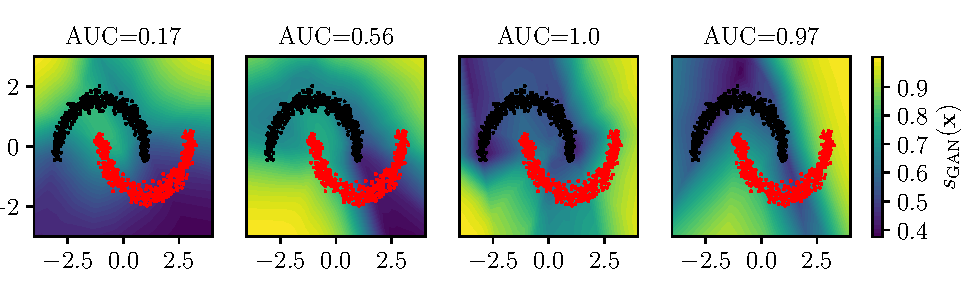
\includegraphics[scale=0.98]{data/chapter_survey/gan_examples.pdf}
\end{centering}
\caption{Four different GAN models trained on the normal (black) data of the \textit{two bananas} dataset, the contours of the respective anomaly scores~\eqref{eq:disc_score} and the AUC of the model with respect to the anomalous (red) data. All the models have the same hyperparameters and yet they converged to very different states.}
\label{fig:gan_examples}
\end{figure}

The idea of using a GAN for anomaly detection comes from the the ability of the generator to learn the true data distribution $p(\vc{x})$ and especially the ability of the discriminator to recognize samples coming from $p(\vc{x})$. When the training dataset consists of normal samples, the discriminator output can be converted into an anomaly score
\begin{equation} \label{eq:disc_score}
     s_{\text{GAN}}(\vc{x}) = 1 - d_{\vc{\varphi}}(\vc{x}),
\end{equation}
which is higher for suspected anomalies and lower for normal data. The common critique is that the discriminator was not trained to recognize an arbitrary distribution of the anomalies but only that of the latent transformed by the generator. Thus it may fail to recognize anomalous samples of interest. Also, the training procedure of a GAN model has very high variance in the sense that two models with the same architecture and hyperparameters and trained on the same data might converge to very different states, see Fig.~\ref{fig:gan_examples}. This implies that more models need to be crated and trained in order to find a good anomaly detector. This is further discussed in Chapter~\ref{sec:chapter_comparison}.

The authors of the \textbf{AnoGAN} model~\cite{schlegl2017unsupervised} recognize some of these flaws. Their convolutional GAN model is trained with the feature-matching loss~\eqref{eq:fmgan}. For identification of anomalies in medical images, instead of using~\eqref{eq:disc_score}, they propose an iterative procedure that searches for the latent code $\vc{z}$ most likely to generate the tested sample to identify anomalous images. However, this procedure is computationally expensive. Therefore, an update to this model was published, the \textbf{f(ast)AnoGAN}~\cite{schleglFAnoGANFastUnsupervised2019}. It uses a Wasserstein GAN~\cite{gulrajani2017improved,haloui2018anomaly} (more on Wasserstein optimization objective in the next section) with gradient penalization~\cite{gulrajani2017improved} to improve training stability and adds an encoder distribution $q_{\phi}(\vc{z}|\vc{x})$ to find $\vc{z}$ closest to given $\vc{x}$ faster. The anomaly score of fAnoGAN is a combination of the discriminator score~\eqref{eq:disc_score} and the feature-matching loss~\eqref{eq:fm_loss}. 

The fmGAN model is used the publication~\cite{kliger2018novelty}, where it is tested on benchmark datasets such as MNIST and CIFAR-10. In~\cite{wang2018generative}, a GAN model was used to detect anomalies in time series data coming from industrial processes, whereas in~\cite{zenatiEfficientGANBasedAnomaly2018}, network intrusions were detected. In the \textbf{Multiple-Objective Generative Adversarial Active Learning} (MOGAAL)~\cite{liu2019generative}, $k \in \mathbb{N}$ generators are trained against a single discriminator on input data divided into $k$ subsets. The discriminator score Eq.~\eqref{eq:disc_score} is used to test new samples. The authors of the OCGAN model~\cite{perera2019ocgan} claim to have achieved state-of-the-art results in one-class classification through severely restricting the latent space of the GAN combined with an autoencoder and employing an adversarial data augmentation strategy. 

The use of GAN with an encoder~\cite{donahue2016adversarial} or an autoencoder with a discriminator~\cite{leveau2017adversarial} for anomaly detection is often and somehow blurs the line between GAN and VAE-based models, but we believe that presenting both concepts separately is useful. True GAN-like models for anomaly detection are however far less prevalent than models that use some autoencoding structure, which will be the focus of the next section. Experimental comparison of both approaches is presented in Chapter~\ref{sec:chapter_comparison}.

\section{VAE-based models} \label{sec:vae_models}
The \textbf{Variational Autoencoder} (VAE) is a generative model that has enjoyed a great success in a number of fields since its introduction in~\cite{kingma2013vae}. Its basic architecture~\cite{kingma2019introduction} is very similar to that of an AE model described in Sec.~\ref{sec:reconstruction_models}, but that is where the similarities end, as VAE is more of a probabilistic anomaly detector, since it models the probability distribution of the normal data. Unlike in AE, where the encoding to latent space $\mathcal{Z}$ is not constrained from taking any shape or form as far as the learning objective is minimized, in VAE a desired distribution of the encodings is explicitly prescribed in the form of a prior distribution $p(\vc{z})$. If the network is trained properly and the encodings follow the prior, we can feed samples from $p(\vc{z})$ to the decoder and expect to obtain random samples in the $\mathcal{X}$ space that will resemble those from the training dataset. This is the simple principle of how VAE works --- more details will be given in the following text.

The VAE has been mainly used for generation of artificial images such as faces~\cite{rezende2014stochastic} or sentences~\cite{bowman2015generating}, but also for other tasks such as semi--supervised learning~\cite{kingma2014semi}, segmentation~\cite{sohn2015learning}, static image forecasting~\cite{walker2016uncertain} and of course for anomaly detection~\cite{an2015variational,xu2018unsupervised,solch2016variational}. Since its popularity, a multitude of approaches enhancing the original VAE has been published, approaching the paradigm from different angles, with some of the more prominent examples published in~\cite{higgins2017beta,zhao2017infovae,tolstikhin2017wasserstein,makhzani2015adversarial,pu2017adversarial}. In the following text, we will go through the basic theory, its implications for the basic VAE, and through some of the extensions. 

\subsection{Basic VAE} \label{sec:vanilla_vae}
Let's begin by defining the VAE from a probabilistic perspective. Assume that there is a dataset $X$ consisting of i.i.d samples. We want to obtain a tractable estimate of the true data distribution $p(\vc{x})$ in order to be able to sample from it. For that purpose, suppose that there is a hidden random process that generates the data and which involves a latent variable $\vc{z}$. Then, like in the case of the GAN model, we can redirect the sampling from the data space $\mathcal{X}$ to the latent space
$\mathcal{Z}$, in which it might be easier. Specifically, we want to sample from the latent prior distribution specified by a density $p(\vc{z})$, then pass this sample to the generative distribution with density $p_{\vc{\theta}}(\vc{x}|\vc{z})$, where $\vc{\theta}$ are its parameters, and obtain a sample $\vc{x}$ that will be very similar to the samples coming from the true data distribution $p(\vc{x})$. In other words, we want to maximize the probability of each sample obtained through the generative process
\begin{equation} \label{eq:vae-px}
p_{\vc{\theta}}(\vc{x})=\int_{\mathcal{Z}}p_{\vc{\theta}}(\vc{x}|\vc{z})p(\vc{z})d\vc{z}.
\end{equation}
Unfortunately, there are several issues with this. Firstly, we do not know the optimal value of parameters $\vc{\theta}$. Secondly, the integral~(\ref{eq:vae-px}) is usually intractable, e.g. in the case where $p_{\vc{\theta}}(\vc{x}|\vc{z})$ is represented by a neural network. Finally, we want to avoid expensive sampling methods such as Monte Carlo Expectation Maximization~\cite{levine2001implementations}. A sampling procedure is eventually used, but we only want to pass such samples $\vc{z}$ to the generative model that will already be very likely under $p_{\vc{\theta}}(\vc{x}|\vc{z})$. To this end, we introduce a discriminative distribution $q_{\vc{\phi}}(\vc{z}|\vc{x})$ which is an approximation of the true intractable posterior $p(\vc{z}|\vc{x})$, with parameters $\vc{\phi}$.

\subsubsection{The ELBO objective}
Now, we would like to relate the generative and discriminative distributions together in way that would enable us to optimize the model with respect to $\vc{\phi},\vc{\theta}$. Continuing from~(\ref{eq:vae-px}),
\begin{equation}
\ln p_{\vc{\theta}}(\vc{x})=\mathbb{E}_{q_{\vc{\phi}}(\vc{z}|\vc{x})}\left[\ln p_{\vc{\theta}}(\vc{x})\right]=\mathbb{E}_{q_{\vc{\phi}}(\vc{z}|\vc{x})}\left[\ln p_{\vc{\theta}}(\vc{x}|\vc{z})+\ln p(\vc{z})-\ln p(\vc{z}|\vc{x})\right],
\end{equation}
where we have used the Bayes' rule and the fact that $p_{\vc{\theta}}(\vc{x})$ does not depend on $\vc{z}$. Now we use the KL divergence~\eqref{eq:kld}
\begin{eqnarray}
\ln p_{\vc{\vc{\theta}}}(\vc{x})-D_{\text{KL}}\left(q_{\vc{\phi}}(\vc{z}|\vc{x})||p(\vc{z}|\vc{x})\right) & = & \mathbb{E}_{q_{\vc{\phi}}(\vc{z}|\vc{x})}\left[\ln p_{\vc{\theta}}(\vc{x}|\vc{z})+\ln p(\vc{z})-\ln q_{\vc{\phi}}(\vc{z}|\vc{x})\right]\label{eq:elbo1}\\
 & = & \mathbb{E}_{q_{\vc{\phi}}(\vc{z}|\vc{x})}\left[\ln p_{\vc{\theta}}(\vc{x}|\vc{z})\right]-D_{\text{KL}}\left(q_{\vc{\phi}}(\vc{z}|\vc{x})||p(\vc{z})\right)\label{eq:elbo2}\\
 & = & - \mathcal{L}_{\text{VAE}}(\vc{x},\vc{\phi},\vc{\theta})\label{eq:elbo3}
\end{eqnarray}
This is the variational lower bound of the VAE model, sometimes called \textbf{ELBO} (evidence lower boundary) through which we can optimize the marginal likelihood $p_{\vc{\theta}}(\vc{x})$. This is due to the fact that the analytically unsolvable term $D_{\text{KL}}\left(q_{\vc{\phi}}(\vc{z}|\vc{x})||p(\vc{z}|x)\right)$ is always nonnegative, thus by maximization of ELBO (minimization of $\mathcal{L}_{\text{VAE}}(\vc{x},\vc{\phi},\vc{\theta})$) we also maximize $p_{\vc{\theta}}(\vc{x})$.

By looking at the individual parts of Eq.~(\ref{eq:elbo2}), we can see that by maximizing the ELBO, we simultaneously maximize the likelihood $p_{\vc{\theta}}(\vc{x}|\vc{z})$ and minimize the distance between $q_{\vc{\phi}}(\vc{z}|\vc{x})$ and $p(\vc{z})$. While looking at the left--hand side of \eqref{eq:elbo1} we can see that at the same time, the marginal likelihood $p_{\vc{\theta}}(\vc{x})$ is maximized and the error term $D_{\text{KL}}\left(q_{\vc{\phi}}(\vc{z}|\vc{x})||p(\vc{z}|\vc{x})\right)$ is minimized, forcing the shape of $q_{\vc{\phi}}(\vc{z}|\vc{x})$ to the true posterior. Also, \eqref{eq:elbo2} captures the autoencoding nature of the VAE model. We pass $\vc{x}$ to the discriminative distribution, which acts as an encoder, sample latent encoding $\vc{z} \sim q_{\vc{\phi}}(\vc{z}|\vc{x})$ and pass this back to generative distribution, which acts as a decoder, to obtain a reconstructed sample $\vc{x}' \sim p_{\vc{\theta}}(\vc{x}|\vc{z})$. From this point on, we will use the term encoder and decoder to describe the discriminative and generative distributions.

\begin{figure}
\centering{}\begin{tikzpicture}
  \node[const]                               (x) {$\vc{x}$};
  \node[const, right = 0.4cm of x]           (xin) {};
  % encoder in
  \node[latent, right = 0.4cm of x, yshift = 0.825cm] (E11) {};
  \node[latent, right = 0.4cm of x, yshift = 0.275cm] (E12) {};
  \node[latent, right = 0.4cm of x, yshift = -0.275cm] (E13) {};
  \node[latent, right = 0.4cm of x, yshift = -0.825cm] (E14) {};
  % encoder hidden
  \node[latent, right = 1.6cm of x, yshift = 0.55cm] (E21) {};
  \node[latent, right = 1.6cm of x, yshift = 0cm] (E22) {};
  \node[latent, right = 1.6cm of x, yshift = -0.55cm] (E23) {};
  % encoder out
  \node[latent, right = 2.8cm of x, yshift = 0.9cm] (E31) {};
  \node[latent, right = 2.8cm of x, yshift = 0.35cm] (E32) {};
  \node[latent, right = 2.8cm of x, yshift = -0.35cm] (E33) {};
  \node[latent, right = 2.8cm of x, yshift = -0.9cm] (E34) {};
  % encoder tag
  \node[const, right = 1.6cm of x, yshift = 1.4cm] (ED) {$q_{\vc{\phi}}(\vc{z}|\vc{x})$};
  % code
  \node[const, right = 3.8cm of x, yshift = 0.575cm]           (mu) {$\vc{\mu}_{\vc{\phi}}$};
  \node[const, right = 3.8cm of x, yshift = -0.575cm]           (sigma) {$\vc{\sigma}^2_{\vc{\phi}}$};
  \node[const, right = -1.0cm of mu]           (muout) {};       
  \node[const, right = -1.0cm of sigma]           (sigmaout) {};       
  \node[const, right = 4.8cm of x, yshift=-0.1cm]           (z) {$z=\mu_{\vc{\phi}}+\sigma_{\vc{\phi}} \odot \varepsilon$};
  \node[const, right = -2.7cm of z]           (zout) {};
  \node[const, right = 4.95cm of x, yshift = 0.9cm]         (epsilon) {$\varepsilon \sim \mathcal{N}(0,\vc{I})$};
  \node[const, right = 5.9cm of x, yshift = 0.2cm]         (epsilonin) {};
  \node[const, right = 0.5cm of z]           (zin) {};
  % decoder in
  \node[latent, right = 0.6cm of z, yshift = 0.275cm] (D11) {};
  \node[latent, right = 0.6cm of z, yshift = -0.275cm] (D12) {};
  % decoder hidden
  \node[latent, right = 1.8cm of z, yshift = 0.55cm] (D21) {};
  \node[latent, right = 1.8cm of z, yshift = 0cm] (D22) {};
  \node[latent, right = 1.8cm of z, yshift = -0.55cm] (D23) {};
  % decoder out
  \node[latent, right = 3cm of z, yshift = 0.825cm] (D31) {};
  \node[latent, right = 3cm of z, yshift = 0.275cm] (D32) {};
  \node[latent, right = 3cm of z, yshift = -0.275cm] (D33) {};
  \node[latent, right = 3cm of z, yshift = -0.825cm] (D34) {};
  % xhat
  \node[const, right = 4cm of z]           (xhat) {$\vc{x}'$};
  \node[const, right = -0.8cm of xhat]       (xhatout) {};    
  % decoder tag
  \node[const, right = 1.6cm of z, yshift = 1.4cm] (DD) {$p_{\vc{\theta}}(\vc{x}|\vc{z})$};   
  
  % edges
  \nedge {x} {xin}
  % encoder 
  \nedge {E11, E12, E13, E14} {E21, E22, E23}
  \nedge {E21, E22, E23} {E31, E32, E33, E34}
  % latent
  \nedge {muout} {mu}
  \nedge {sigmaout} {sigma}
  \nedge {mu,sigma} {zout}
  \nedge {z} {zin}
  \nedge {epsilon} {epsilonin}
  % decoder
  \nedge {D11, D12} {D21, D22, D23}
  \nedge {D21, D22, D23} {D31, D32, D33, D34} 
  %xhat
  \nedge {xhatout} {xhat}
\end{tikzpicture}

\caption{A schematic of a Variational Autoencoder consisting of fully connected layers with a Gaussian encoder $q_{\vc{\phi}}(\vc{z}|\vc{x})$ with mean $\vc{\mu}_{\vc{\phi}}$ and variance $\vc{\sigma}^2_{\vc{\phi}}$, which are extracted from the last layer of the encoder. They are used to sample an encoding $\vc{z}$ through the reparametrization trick with a noise variable $\varepsilon$. The encoding is then passed forward and the reconstruction $\vc{x}'$ is sampled from the decoder $p_{\vc{\theta}}(\vc{x}|\vc{z})$.}
\label{fig:vae}
\end{figure}

\subsubsection{Vanilla VAE}
To be able to optimize~\eqref{eq:elbo3}, we must make some additional assumptions about the model. Here, we will describe those that were made by the authors of the original "vanilla" VAE model, but note that different choices are also possible. First, the \textbf{prior} $p(\vc{z})$ is chosen to be an $h$-dimensional unit normal distribution $p(\vc{z})=\mathcal{N}(\vc{z}|0,\textbf{I})$. The encoded training data are expected to follow this distribution after optimization and it is used for generation of new samples. In tandem with this, the encoder is assumed to model a normal distribution with diagonal covariance matrix $q_{\vc{\phi}}(\vc{z}|\vc{x})=\mathcal{N}\left(\vc{z}|\mu_{\vc{\phi}}(x), \text{diag}(\vc{\sigma}^2_{\vc{\phi}}(x))\right), \vc{\mu}_{\vc{\phi}}, \vc{\sigma}^2_{\vc{\phi}}:\mathbb{R}^d \rightarrow \mathbb{R}^h$, where the mean and variance estimates are computed by neural networks with shared weights $\vc{\phi}$. These choices lead to an analytically solvable expression for the KL divergence in~\eqref{eq:elbo2}, see~\eqref{eq:kl_standard} in the Appendix
\begin{equation} \label{eq:vae_kld}
D_{\text{KL}}\left(q_{\vc{\phi}}(\vc{z}|\vc{x})||p(\vc{z}) \right) = \frac{1}{2}\sum_{i=1}^{d} 1-\sigma_{\vc{\phi},i}^{2}(\vc{x})+\ln \sigma_{\vc{\phi},i}^{2}(\vc{x}) -\mu_{\vc{\phi},i}^{2}(\vc{x}).
\end{equation}

Second, the optimization of the ELBO~\eqref{eq:elbo3} requires sampling from the encoder $q_{\vc{\phi}}(\vc{z}|\vc{x})$. This is however problematic for optimization by backpropagation, because sampling is not a differentiable operation. Therefore, a \textbf{reparametrization trick} was introduced in~\cite{kingma2013vae}. Instead of directly drawing samples from $q_{\vc{\phi}}(\vc{z}|\vc{x})$, we first take a sample from an $h$-dimensional noise distribution $\varepsilon\sim p(\varepsilon)=\mathcal{N}(0,\mathbf{I})$ and then compute the encoding as $\vc{z}=\vc{\mu}_{\vc{\phi}}(\vc{x})+\vc{\sigma}_{\vc{\phi}}(\vc{x}) \odot \varepsilon$, where $\odot$ denotes element-wise multiplication. This changes the first term of the ELBO, which is called the \textbf{log-likelihood} to
\begin{equation} \label{eq:vae_reparam}
\mathbb{E}_{q_{\vc{\phi}}(\vc{z}|\vc{x})}\left[\ln p_{\vc{\theta}}(\vc{x}|\vc{z})\right] = \mathbb{E}_{\varepsilon\sim\mathcal{N}(0,\textbf{I})}\left[\ln p_{\vc{\theta}}(\vc{x}| \vc{\mu}_{\vc{\phi}}(\vc{x})+\vc{\sigma}_{\vc{\phi}}(\vc{x}) \odot \varepsilon )\right].
\end{equation}
In the following text, whenever it can apply, we use the notation $\vc{z} \sim q_{\vc{\phi}}(\vc{z}|\vc{x})$ as a shorthand for the reparametrization trick.

Finally, the decoder $p_{\vc{\theta}}(\vc{x}|\vc{z})$ is also assumed to model a normal distribution\\ $\mathcal{N}(\vc{x}|\vc{\mu}_{\vc{\theta}}(\vc{z}),\sigma^2 I), \vc{\mu}_{\vc{\theta}} :\mathbb{R}^h \rightarrow \mathbb{R}^d, \sigma^2\in\mathbb{R}^+$, although a Bernoulli distribution is sometimes used for data scaled to the interval [0,1]. The mean of the decoder distribution is again represented by a neural network with weights $\vc{\theta}$. The variance parameter $\sigma^2$ is either fixed, or it can be estimated from data during training. Therefore, the log-likelihood takes on the form 
\begin{equation} \label{eq:vae_logpx}
\ln p_{\vc{\theta}}(\vc{x}|\vc{z}) = - \frac{1}{2\sigma^2} \vert \vert \vc{x} - \vc{\mu}_{\vc{\theta}}(\vc{z}) \vert \vert_2^2 - \frac{d}{2} \ln 2\pi - d \ln \sigma. 
\end{equation}
Note that the last two terms can be left out of the optimization, since they are not dependent on any inputs or weights. Again, we see the connection with an autoencoding model, where the log-likelihood~\eqref{eq:vae_logpx} has very similar form to the objective~\eqref{eq:ae_objective}. Here, the reconstruction takes the form of $\vc{x}' = \vc{\mu}_{\vc{\theta}}(\vc{z})$. A notable property of the VAE model is that the reconstruction is stochastic, which is due to the sampling used in the reparametrization trick~\eqref{eq:vae_reparam}. 

Now, we combine the assumptions and equations~\eqref{eq:vae_kld}--\eqref{eq:vae_logpx} to derive the final analytic form of the ELBO objective. The expectation in~\eqref{eq:vae_reparam} is replaced by a mean of $L$ sample of $z$ through the reparametrization trick. The VAE loss function, that is minimized with respect to $\vc{\phi}, \vc{\theta}$, and which is in fact equal to negative ELBO~\eqref{eq:elbo3}, has the form
\begin{equation} \label{eq:vae_loss}
\mathcal{L_{\text{VAE}}}(\vc{x},\vc{\phi},\vc{\theta})=\frac{1}{2\sigma^2 L}\sum_{l=1}^{L}||\vc{x}-\vc{\mu}_{\vc{\theta}}(\vc{z}^{l})||_{2}^{2} - \frac{1}{2}\sum_{i=1}^{d} 1-\sigma_{\vc{\phi},i}^{2}(x)+\ln\sigma_{\vc{\phi},i}^{2}(x)-\mu_{\vc{\phi},i}^{2}(x),
\end{equation}
\begin{equation} 
\vc{z}^l=\vc{\mu}_{\vc{\phi}}(\vc{x})+\vc{\sigma}_{\vc{\phi}}(\vc{x}) \odot \varepsilon^l, \varepsilon^l \sim  \mathcal{N}(0,\mathbf{I}). \nonumber
\end{equation}
This can be directly optimized via gradient descent techniques. We set $L=1$ in accordance with~\cite{kingma2013vae}. See Fig.~\ref{fig:vae} for a schematic example of a VAE model. The training procedure of a VAE is described in Alg.~\ref{alg:vae_train}. An example of the outputs of a VAE model trained on the MNIST hand--written digits dataset~\cite{lecun-mnisthandwrittendigit-2010} is in Fig.~\ref{fig:mnist_reconstruction}.

\begin{algorithm}
\begin{algorithmic}[1]
\Require{A VAE model with encoder $q_{\vc{\phi}}(\vc{z}|\vc{x})$ and decoder $p_{\vc{\theta}}(\vc{x}|\vc{z})$, training set $X=\lbrace \vc{x}_1, \vc{x}_2, \ldots, \vc{x}_n \rbrace \subset \mathcal{X}$, maximum number of iterations $I\in\mathbb{N}$, batchsize $B \in \mathbb{N}$.}
\State $\vc{\phi},\vc{\theta} \gets $ Initialize parameters
\State{$i \gets $ Iteration counter}
\While{$i<I$ or $\vc{\phi},\vc{\theta}$ are not converged}
	\State{$X_B \gets$ A random batch of $B$ samples from $X$}
	\State$l \gets \frac{1}{B}\sum_{j=1}^L \mathcal{L}_\text{VAE}(\vc{x}_j,\vc{\phi},\vc{\theta}), \vc{x}_j \in X_B$
	\State$\vc{\phi} \stackrel{+}\gets - \nabla_{\vc{\phi}}l $ update of encoder weights
	\State$\vc{\theta} \stackrel{+}\gets - \nabla_{\vc{\theta}}l $ update of decoder weights
	\State{$i \gets i+1$}
\EndWhile
\State{\textbf{return} encoder $q_{\vc{\phi}}(\vc{z}|\vc{x})$, decoder $p_{\vc{\theta}}(\vc{x}|\vc{z})$}
\end{algorithmic}\caption{Variational Autoencoder training procedure.}
\label{alg:vae_train}
\end{algorithm}

\begin{figure}
\centering{}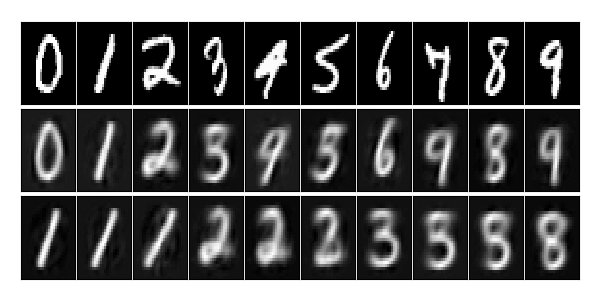
\includegraphics[scale=0.8]{data/chapter_survey/mnist_reconstruction_generation}\caption{Example of a simple VAE trained on the MNIST dataset. Here, the neural networks modelling the encoder and decoder parameters contained two levels of convolutional blocks. Ground truth examples are in the top row, reconstructed samples are in the middle row, artificially generated digits are in the bottom row. The reconstructions are blurry, which is a typical VAE behaviour. Also, the reconstruction is imperfect for digits which resemble each other, such as "9", "4" and "7", or "3" and "8". The artificial digits were created by linearly interpolating between two coordinates in the latent space and using this as an input to the decoder. The VAE then produces a smooth interpolation between digits "1" and "8" that contains the related digits "2" and "3".}
\label{fig:mnist_reconstruction}
\end{figure}
 
\subsubsection{Some VAE properties}
\begin{figure}
\begin{centering}
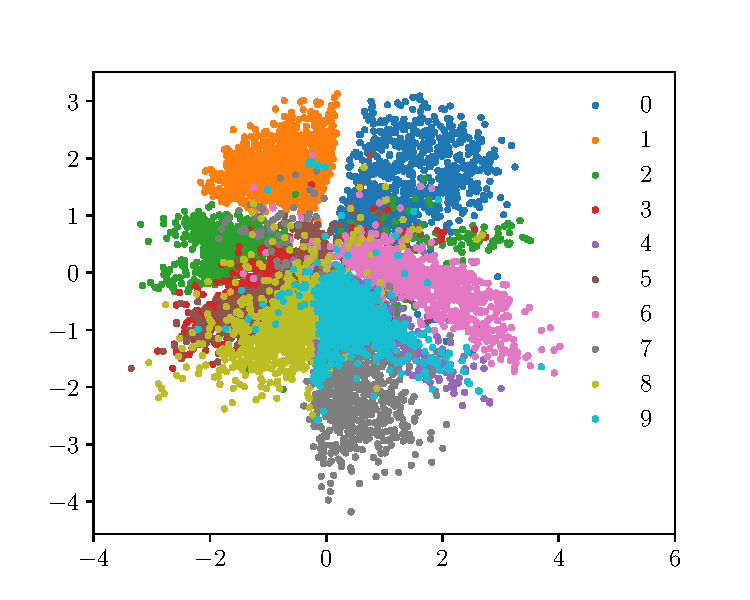
\includegraphics[scale=0.8]{data/chapter_survey/mnist_latent}
\par\end{centering}
\caption{The latent space of the MNIST dataset produced by a VAE with a two-dimensional latent space. Note the overlapping of some digit encodings, e.g. "7" and "9".}
\label{fig:mnist_latent}
\end{figure}

If a VAE model is correctly trained, we can assume that the encoder $q_{\vc{\phi}}(\vc{z}|\vc{x})$ and prior $p(\vc{z})=\mathcal{N}(\vc{z}|0,\textbf{I})$ are close to each other. Then, samples from the prior can be fed to the decoder and one can expect artificial samples that resemble the training data. A \textbf{generated sample} can therefore be described as
\begin{equation} \label{eq:generated_sample}
    \tilde{\vc{x}} = \vc{\mu}_{\vc{\theta}}(\vc{z}), \vc{z} \sim p(\vc{z}).
\end{equation}
Note that a \textbf{reconstructed sample} is instead obtained by sampling the encoding $\vc{z}$ from the encoder through the reparametrization trick~\eqref{eq:vae_reparam}. This is also a place to note why we are using neural network representation of the encoder and decoder. Since neural networks have be proven to be universal function approximators, we know that given enough capacity, data and training time, the decoder can learn a mapping from the prior to an arbitrary function.

\begin{figure}
\centering
    \begin{subfigure}[b]{0.45\textwidth}
        \centering
        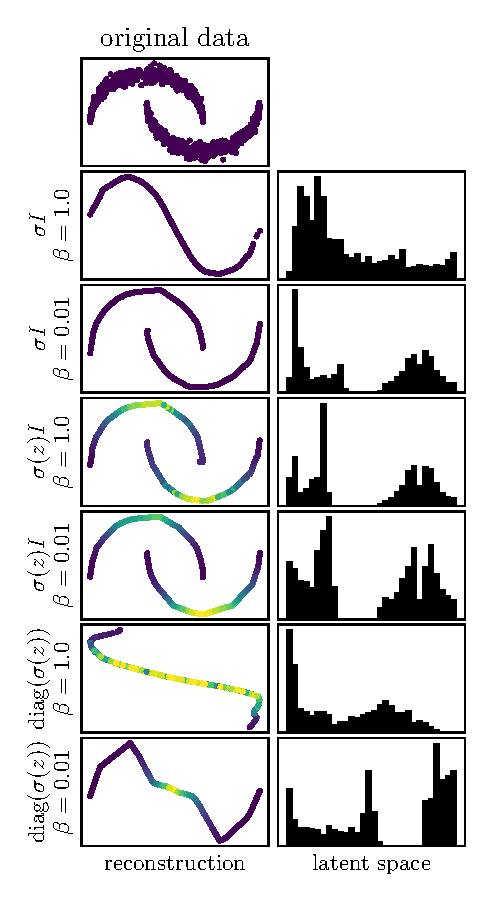
\includegraphics[scale=0.9]{data/chapter_survey/vae_two_moons_z1_colored}
        \caption{$h=1$}
    \end{subfigure}
    \begin{subfigure}[b]{0.45\textwidth}
        \centering
        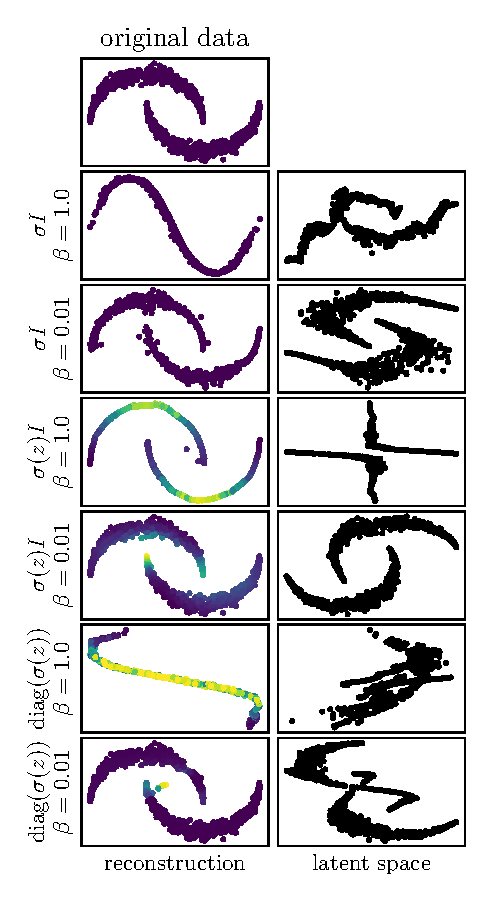
\includegraphics[scale=0.9]{data/chapter_survey/vae_two_moons_z2_colored}
        \caption{$h=2$}
    \end{subfigure}
\caption{An overview of VAE behaviour with respect to the scaling parameter $\beta$ of the objective~\eqref{eq:betavae} and to the way the covariance of the decoder $p_{\vc{\theta}}(\vc{x}|\vc{z})$ is estimated. The VAE model was trained on the two--moons data, plotted in the plots at the very top. Variants with 1D (a) and 2D (b) latent spaces are compared, means of the decoder $\vc{\mu}_{\vc{\theta}}(\vc{z})$ are plotted on the left and the latent representations on the right. Clearly, smaller values of $\beta$ lead to better sample reconstruction, especially in the case of a two-dimensional latent space, as well as leading to a better separation of the encodings. This is understandable, since the prior $p(\vc{z})=\mathcal{N}(0,\textbf{I})$ is unimodal. From the top: the covariance of the decoder is given either by a fixed scalar ($\sigma^2 I,\sigma=1$), by a scalar estimated from the data ($\sigma^2(\vc{z})I$), or by an estimate of its diagonal terms ($\text{diag}(\sigma^2(\vc{z}))$). The magnitude of the estimated variance in the two latter cases is denoted by color, where a brighter color corresponds to a higher value of variance. It is interesting that the second case ($\sigma^2(\vc{z})I$) seems to alleviate the reconstruction difficulties with higher $\beta$, while the estimation of the full covariance diagonal does not exhibit such property. Also, the third case seems to "exploit" the estimation of variance. Instead of pushing and optimizing the mean, it can instead simply put higher variance in the direction in which the reconstruction is worse and still incur only a small loss. Due to this behaviour, the second case seems to be the most robust and stable way of estimation of the reconstruction variance. Not surprisingly, the 2D case provides better reconstructions since it was provided with one more dimension to encode data to.}
\label{fig:betavae}
\end{figure}

Fig.~\ref{fig:mnist_latent} shows the latent space of an example VAE model. Note that although the overall distribution of the encodings resembles the normal prior, in order to be able to reconstruct the samples from the encodings, the model has to learn to encode the samples from different digit classes to different parts of the latent space. It was shown~\cite{higgins2017beta} that the reconstruction and regularization parts of the VAE loss~\eqref{eq:elbo3} actually work against each other. A model with encoder perfectly copying the randomness of the prior would not be able to reconstruct the inputs. On the other hand, a model without the latent regularization would not be able to generate new samples, as it would be practically identical with an AE model from Sec.~\ref{sec:reconstruction_models}, which is free to encode the different classes to arbitrary parts of the latent space. The basic loss~\eqref{eq:vae_loss} leads to a model that is usually in an equilibrium between both of these states. It is however possible to push the model in one of these directions by using a scaling parameter
\begin{equation} \label{eq:betavae}
\mathcal{L}_{\beta\text{VAE}}(\vc{x},\vc{\phi},\vc{\theta},\beta)= - \mathbb{E}_{q_{\vc{\phi}}(\vc{z}|\vc{x})}\left[\ln p_{\vc{\theta}}(\vc{x}|\vc{z})\right] + \beta D_{\text{KL}}\left(q_{\vc{\phi}}(\vc{z}|\vc{x})||p(\vc{z})\right),\beta>0.
\end{equation}
A VAE model trained with this loss is known as \textbf{BetaVAE}~\cite{higgins2017beta} and is one of the first VAE-based models that attempt some sort of \textbf{unsupervised disentanglement}. A disentangled model captures the possible factors of variation of a dataset in orthogonal dimensions of the latent space. Imagine a colored MNIST dataset, on which a disentangled model with a two dimensional latent space is trained. If properly disentangled, one latent dimension would capture the identity of the digit, while the other one would capture its color. This concept will be again revisited in Chapter~\ref{sec:chapter_sgvaegan}. The influence of the $\beta$ parameter is discussed in Fig.~\ref{fig:betavae}.

Instead of setting a fixed variance parameter $\sigma^2$ in the decoder, one can optimize and extract it instead from the last layer of the decoder, either as a scalar $\sigma^2_{\vc{\theta}}(\vc{z}) \in \mathbb{R}^+$
or even a full diagonal of the covariance $\text{diag}\left(\vc{\sigma}^2_{\vc{\theta}}(\vc{z})\right),\vc{\sigma}^2_{\vc{\theta}}(\vc{z})\in\mathbb{R}^{d+}$. From the experiment in Fig.~\ref{fig:betavae}, it seems (at least for tabular data) that the best results were surprisingly obtained not by the most complex variant, but the one with a scalar value $\sigma^2_{\vc{\theta}}$ optimized during training.

\subsection{Wasserstein and adversarial autoencoders} \label{sec:wae}
The asymmetry of the KL divergence motivated search for a more accurate metric measuring the distance between the prior and the encoder. An alternative approach to VAE has been published in~\cite{mescheder2017adversarial} and improved in~\cite{tolstikhin2017wasserstein}, which proposes a general form of a generative autoencoder that uses a Wasserstein metric~\cite{givens1984class}. Unlike the KL divergence term in the VAE loss, which forces all the input data samples to zero (the mean of the standard prior), in \textbf{Wasserstein autoencoders} (WAE) the encoding is loosened, which reportedly leads to improved reconstruction~\cite{tolstikhin2017wasserstein}. A general form of the loss function of a WAE model is
\begin{equation} \label{eq:general_wae_loss}
    \mathcal{L}_{\text{DW}} (\vc{x}, \vc{\theta}, \vc{\phi}) = - \mathbb{E}_{q_{\vc{\phi}}(\vc{z}|\vc{x})} \left[ \ln p_{\vc{\theta}}(\vc{x}|\vc{z}) \right] + \lambda D_{\text{W}} \left( q_{\vc{\phi}}(\vc{z}|\vc{x}) || p(\vc{z}) \right),
\end{equation}
where $\lambda >0$  is a scalar hyperparameter, and $D_{\text{W}}$ is a Wasserstein metric. The most commonly used form of the Wasserstein metric is the kernelized \textbf{maximum-mean-discrepancy} (MMD) with a kernel function $k_f:\mathbb{R}^h \times \mathbb{R}^h \rightarrow \mathbb{R}$, which was reported to perform well in matching high dimensional distributions~\cite{zhao2017infovae}. From the theoretical point of view, KLD only matches the first and the second moment of the two distributions, while MMD can potentially match an infinite amount of moments with the right kernel. Some authors~\cite{tolstikhin2017wasserstein} argue that by minimizing KLD, the latent representation might become uninformative for the decoder to reconstruct the code. On the other hand, MMD maximizes the mutual information between $\vc{x}$  and $\vc{z}$~\cite{zhao2017infovae}.

\begin{algorithm}
\begin{algorithmic}[1]
\Require{A WAE model with encoder $q_{\vc{\phi}}(\vc{z}|\vc{x})$, decoder $p_{\vc{\theta}}(\vc{x}|\vc{z})$ and a prior $p(\vc{z})$, training set $X=\lbrace \vc{x}_1, \vc{x}_2, \ldots, \vc{x}_n \rbrace \subset \mathcal{X}$, maximum number of iterations $I\in\mathbb{N}$, batchsize $B \in \mathbb{N}$, regularization coefficient $\lambda > 0$, characteristic positive definite kernel $k_f$, standard deviation parameter $\sigma$ > 0.}
\State $\vc{\phi},\vc{\theta} \gets $ Initialize parameters
\State{$i \gets $ Iteration counter}
\While{$i<I$ or $\vc{\phi},\vc{\theta}$ are not converged}
	\State{$X_B \gets$ A random batch of $B$ samples from $X$}
	\State{$Z \gets \lbrace \vc{z}_j \sim q_{\phi}(\vc{z}|\vc{x}_j), \vc{x}_j \in X_B \rbrace$ samples from the encoder}
	\State{$\tilde{Z} \gets$ A random batch of $B$ samples from prior $p(\vc{z})$}
	\State$l \gets \frac{1}{B}\sum_{j=1}^B  ||\vc{x}_j-\vc{\mu}_{\vc{\theta}}(\vc{z}_j)||_{2}^{2} +\lambda \text{MMD}_k(Z,\tilde{Z}), \vc{x}_j \in X_B, \vc{z}_j \in Z$
	\State$\vc{\phi} \stackrel{+}\gets - \nabla_{\vc{\phi}}l $ update of encoder weights
	\State$\vc{\theta} \stackrel{+}\gets - \nabla_{\vc{\theta}}l $ update of decoder weights
	\State{$i \gets i+1$}
\EndWhile
\State{\textbf{return} encoder $q_{\vc{\phi}}(\vc{z}|\vc{x})$, decoder $p_{\vc{\theta}}(\vc{x}|\vc{z})$}
\end{algorithmic}
\caption{Wasserstein autoencoder training procedure.}
\label{alg:infovae}
\end{algorithm}

Under some mild assumptions about the kernel function $k_f$, which needs to be characteristic and positive-definite (see details in~\cite{tolstikhin2017wasserstein}), the MMD can be expressed in such a way that enables optimization of the model by backpropagation. Then, the MMD of the prior and the encoder can be approximated solely by comparing sets of samples from these distributions $Z=\{\vc{z}_{1}, \vc{z}_{2}, \ldots, \vc{z}_{n}\}, \tilde{Z}=\{\tilde{\vc{z}}_{1}, \tilde{\vc{z}}_{2}, \ldots, \tilde{\vc{z}}_{n}\},\vc{z}_{i}\sim q_{\vc{\phi}}(\vc{z}|\vc{x}),\tilde{\vc{z}}_{i} \sim p(\vc{z}),\forall i \in \hat{n}$ in a closed expression
\begin{equation} \label{eq:mmd}
\text{MMD}_{k}(Z,\tilde{Z})=\frac{1}{n(n-1)}\sum_{i\neq j}k_f(\vc{z}_{i},\vc{z}_{j})+\frac{1}{n(n-1)}\sum_{i\neq j}k_f(\tilde{\vc{z}}_{i},\tilde{\vc{z}}_{j})-\frac{2}{n^{2}}\sum_{i,j}k_f(\vc{z}_{i}, \tilde{\vc{z}}_{j}).
\end{equation}
The most notable characteristic of the MMD is that in practice, it only requires samples from the distributions in question, and it is therefore less restricting than the KLD, which required normal prior and encoder in order to obtain the analytic expression~\eqref{eq:vae_kld}. This offers the potential for the use of a variety of prior and encoder distributions, however, the reparametrization trick~\eqref{eq:vae_reparam} or a similar technique must be used in order to keep the sampling from $q_{\vc{\phi}}(\vc{z}|\vc{x})$ a differentiable operation. The two most common choices of $k_f$ are the RBF $k_f(\vc{z},\tilde{\vc{z}}) = \exp(- \gamma \vert \vert \vc{z} - \tilde{\vc{z}} \vert \vert_2^2), \gamma > 0$ and inverse multiquadratics (IMQ) $k_f(\vc{z},\tilde{\vc{z}}) = (c^2 +  \vert \vert \vc{z} - \tilde{\vc{z}} \vert \vert_2^2)^\beta, c>0, \beta < 0$ kernels. The training algorithm for a WAE with the MMD is in Alg.~\ref{alg:infovae}. Note that although the parameters $\vc{\phi}$ do not appear  explicitly in the overall loss function, they are present through the samples in $Z$. 

A different architecture arises when the \textbf{Jensen--Shannon divergence} $D_{\text{JS}}$~\cite{barranco1994texture} is used in place of $D_{\text{W}}$. The JSD is a symmetrical (unlike KL divergence) measure of distance between two probability distributions. The use of JSD leads to a model that is called  the \textbf{adversarial autoencoder} (AAE) and was originally proposed in~\cite{makhzani2015adversarial}. The connection between an AAE model and the general formulation~\eqref{eq:general_wae_loss} was shown in~\cite{tolstikhin2017wasserstein}. To regularize the encoder, we add a discriminator $d_{\vc{\eta}}(\vc{z}):\mathcal{Z}\rightarrow\left[0,1\right]$ represented by a neural network with parameters $\vc{\eta}$. The discriminator has a similar function to the one in the GAN model from Sec.~\ref{sec:gan_models}. It tries to recognize latent space samples produced by the encoder and those sampled from the prior $p(\vc{z})$. The difference is that here, the discriminator operates on the latent space $\mathcal{Z}$ instead of the data space $\mathcal{X}$. 

\begin{figure}
\centering{}\begin{tikzpicture}
  \node[const]                               (x) {$\vc{x}$};
  \node[const, right = 0.3cm of x]           (xin) {};
  % encoder in
  \node[latent, right = 0.4cm of x, yshift = 0.825cm] (E11) {};
  \node[latent, right = 0.4cm of x, yshift = 0.275cm] (E12) {};
  \node[latent, right = 0.4cm of x, yshift = -0.275cm] (E13) {};
  \node[latent, right = 0.4cm of x, yshift = -0.825cm] (E14) {};
  % encoder hidden
  \node[latent, right = 1.6cm of x, yshift = 0.55cm] (E21) {};
  \node[latent, right = 1.6cm of x, yshift = 0cm] (E22) {};
  \node[latent, right = 1.6cm of x, yshift = -0.55cm] (E23) {};
  % encoder out
  \node[latent, right = 2.8cm of x, yshift = 0.275cm] (E31) {};
  \node[latent, right = 2.8cm of x, yshift = -0.275cm] (E32) {};
  % encoder tag
  \node[const, right = 1.4cm of x, yshift = 1.1cm] (E) {$q_{\vc{\phi}}(\vc{z}|\vc{x})$};
  % placement
  \node[const, right = 5.2cm of x, yshift=1.2cm]           (encoderin) {}; 
  \node[const, right = 5.2cm of x, yshift=-1.2cm]           (discriminatorin) {}; 
  % code
  \node[const, right = 4.1cm of x, yshift = 0cm]           (zg) {$\vc{z}$};
  \node[const, right = 3.4cm of x]           (zgout) {}; 
  \node[const, right = 0cm of encoderin]           (zgin) {};
  \node[const, right = 0.05cm of zg]           (zgout2) {};
  \node[const, right = 0cm of discriminatorin,yshift=0.05cm]           (zgin2) {};
  % prior
  \node[const, right = -1.8cm of discriminatorin, yshift = 0cm]         (z) {$\tilde{\vc{z}} \sim p(\vc{z})$};
  \node[const, right = 0cm of z, yshift = 0cm]         (zout) {};
  \node[const, right = 0cm of discriminatorin]           (zin) {};

  % decoder in
  \node[latent, right = 0.1cm of encoderin, yshift = 0.275cm] (D11) {};
  \node[latent, right = 0.1cm of encoderin, yshift = -0.275cm] (D12) {};
  % decoder hidden
  \node[latent, right = 1.3cm of encoderin, yshift = 0.55cm] (D21) {};
  \node[latent, right = 1.3cm of encoderin, yshift = 0cm] (D22) {};
  \node[latent, right = 1.3cm of encoderin, yshift = -0.55cm] (D23) {};
  % decoder out
  \node[latent, right = 2.5cm of encoderin, yshift = 0.825cm] (D31) {};
  \node[latent, right = 2.5cm of encoderin, yshift = 0.275cm] (D32) {};
  \node[latent, right = 2.5cm of encoderin, yshift = -0.275cm] (D33) {};
  \node[latent, right = 2.5cm of encoderin, yshift = -0.825cm] (D34) {};
  % xhat
  \node[const, right = 3.4cm of encoderin]           (xhat) {$\vc{x}'$};
  \node[const, right = -0.8cm of xhat]       (xhatout) {};    
  % decoder tag
  \node[const, right = 1.1cm of encoderin, yshift = 1.1cm] (D) {$p_{\vc{\theta}}(\vc{x}|\vc{z})$};   
  
  % discriminator
  \node[latent, right = 0.1cm of discriminatorin, yshift = 0.275cm] (DI11) {};
  \node[latent, right = 0.1cm of discriminatorin, yshift = -0.275cm] (DI12) {};
  % discriminator hidden
  \node[latent, right = 1.3cm of discriminatorin, yshift = 0.55cm] (DI21) {};
  \node[latent, right = 1.3cm of discriminatorin, yshift = 0cm] (DI22) {};
  \node[latent, right = 1.3cm of discriminatorin, yshift = -0.55cm] (DI23) {};
  % discriminator out
  \node[latent, right = 2.5cm of discriminatorin, yshift = 0cm] (DI31) {};
  % xhat
  \node[const, right = 3.45cm of discriminatorin]           (dx) {$s \in [0,1]$};
  \node[const, right = -1.9cm of dx]       (dxout) {};       
  % discriminator tag
  \node[const, right = 1.1cm of discriminatorin, yshift = 1.1cm] (D) {$d_{\vc{\eta}}(\vc{z})$};

  % edges
  \nedge {x} {xin}
  % encoder 
  \nedge {E11, E12, E13, E14} {E21, E22, E23}
  \nedge {E21, E22, E23} {E31, E32}
  % latent
  \nedge {zgout} {zg}
  \nedge {zgout2} {zgin}
  \nedge {zgout2} {zgin2}
  \nedge {zout} {zin}

  % decoder
  \nedge {D11, D12} {D21, D22, D23}
  \nedge {D21, D22, D23} {D31, D32, D33, D34} 
  % discriminator
  \nedge {DI11, DI12} {DI21, DI22, DI23}
  \nedge {DI21, DI22, DI23} {DI31}
  %xhat
  \nedge {xhatout} {xhat}
  %xhat
  \nedge {dxout} {dx}

\end{tikzpicture}
\caption{A schematic of a AAE model consisting of fully connected layers. A data sample $x$ is mapped to latent space representation $\tilde{z}$ via the encoder $q_{\vc{\phi}}(\vc{z}|x)$. Also, a sample $z$ is sampled from the latent prior $p(\vc{z})$. Both $z$ and $\tilde{z}$ are passed to the discriminator $d_{\eta}(\vc{z})$ that produces a score $s$ -- the probability that the input sample comes from the prior. At the same time, the latent representation is passed to the decoder $p_{\vc{\theta}}(x|z)$ which maps it to a reconstruction $\tilde{x}$.}
\label{fig:aae}
\end{figure}

\begin{algorithm}
\begin{algorithmic}[1]
\Require{An AAE model with encoder $q_{\vc{\phi}}(\vc{z}|\vc{x})$, decoder $p_{\vc{\theta}}(\vc{x}|\vc{z})$,  a prior $p(\vc{z})$ and a discriminator $d_{\vc{\eta}}(\vc{z})$, training set $X=\lbrace \vc{x}_1, \vc{x}_2, \ldots, \vc{x}_n \rbrace \subset \mathcal{X}$, maximum number of iterations $I\in\mathbb{N}$, batchsize $B \in \mathbb{N}$, regularization coefficient $\lambda > 0$, standard deviation parameter $\sigma$ > 0.}
\State $\vc{\phi},\vc{\theta}, \vc{\eta} \gets $ Initialize parameters
\State{$i \gets $ Iteration counter}
\While{$i<I$ or $\vc{\phi},\vc{\theta},\vc{\eta}$ are not converged}
	\State{$X_B \gets$ A random batch of $B$ samples from $X$}
	\State{$Z \gets \lbrace \vc{z}_j \sim q_{\vc{\phi}}(\vc{z}|\vc{x}_j), \vc{x}_j \in X_B \rbrace$ samples from the encoder}
	\State{$\tilde{Z} \gets$ A random batch of $B$ samples from prior $p(\vc{z})$}
	\State{$\tilde{X} \gets \lbrace\tilde{\vc{x}}_j \sim p_{\vc{\theta}}(\vc{x}|\tilde{\vc{z}}_j), \tilde{\vc{z}}_j \in \tilde{Z}_B \rbrace$ generated samples}
	\State$l_{ae} \gets \frac{1}{B}\sum_{j=1}^B \mathcal{L}_{\text{AAE}}( \vc{x}_j,\vc{z}_j,\tilde{\vc{z}}_j, , \vc{\theta}, \vc{\phi} ) , x_j \in X_B, \vc{z}_j \in Z, \tilde{\vc{z}}_j \in \tilde{Z}$
	\State{$l_d \gets \frac{1}{B}\sum_{j=1}^B \mathcal{L}_{\text{AAE}_d}(\vc{z}_j,\tilde{\vc{z}}_j, \vc{\eta}), \vc{z}_j \in Z, \tilde{\vc{z}}_j \in \tilde{Z}$}
	\State$\vc{\phi} \stackrel{+}\gets - \nabla_{\vc{\phi}}l_{ae} $ update of encoder weights
	\State$\vc{\theta} \stackrel{+}\gets - \nabla_{\vc{\theta}}l_{ae} $ update of decoder weights
	\State$\vc{\eta} \stackrel{+}\gets - \nabla_{\vc{\eta}}l_{d} $ update of discriminator weights
	\State{$i \gets i+1$}
\EndWhile
\State{\textbf{return} encoder $q_{\vc{\phi}}(\vc{z}|\vc{x})$, decoder $p_{\vc{\theta}}(\vc{x}|\vc{z})$, discriminator $d_{\vc{\eta}}(\vc{z})$}
\end{algorithmic}
\caption{AAE training procedure.}
\label{alg:aae}
\end{algorithm}

A modified loss~\eqref{eq:disc_loss} is used to train the discriminator, while the loss function~\eqref{eq:gen_loss} is used in place of the general Wasserstein distance in~\eqref{eq:general_wae_loss} for training of the encoder and decoder. Explicitly,
\begin{equation} \label{eq:aae_loss_disc}
\mathcal{L}_{\text{AAE}_d}(\vc{z},\tilde{\vc{z}}, \vc{\eta})= - \ln d_{\eta}(\vc{z}) - \ln(1-d_{\vc{\eta}}(\tilde{\vc{z}})),
\end{equation}
\begin{equation} \label{eq:aae_loss_autoencoder}
\mathcal{L}_{\text{AAE}}(\vc{x},\vc{z},\tilde{\vc{z}}, \vc{\theta}, \vc{\phi}) = \frac{1}{\sigma^2}||\vc{x}-\vc{\mu}_{\vc{\theta}}(\vc{z})||_{2}^{2} -\lambda\ln d_{\vc{\eta}}(\tilde{\vc{z}}),
\end{equation}
where $\lambda>0$, $\vc{z} \sim q_{\vc{\phi}}(\vc{z}|\vc{x})$, $\tilde{\vc{z}} \sim p(\vc{z})$. Not that the loss~\eqref{eq:aae_loss_autoencoder} has implicit functional dependence on $\vc{\phi}$ through the samples $\vc{z}$.  A schematic of the AAE model is in Fig.~\ref{fig:aae} and the AAE training procedure is described in Alg.~\ref{alg:aae}. Again, any prior $p(\vc{z})$ that we can sample from is suitable for the regularization of AAE, even a multimodal one. In practice, an AAE model compared to a WAE behaves similarly as GAN compared to VAE. The adversarial loss leads to less blurry reconstructions and generated samples at the cost of higher training instability~\cite{tolstikhin2017wasserstein}. One way to gain advantages of both is to use an AAE architecture as depicted in Fig.~\ref{fig:aae} and add the MMD regularization term~\eqref{eq:mmd} to the loss~\eqref{eq:aae_loss_autoencoder}.

The single-mode prior $p(\vc{z})$ of the VAE model stimulates the distribution $q_{\vc{\phi}}(\vc{z}|\vc{x})$ to have a single mode as well, and therefore it is hard to fit data with a multi-modal latent distribution. The publication~\cite{tomczak2018vae} proposes a learnable multimodal \textbf{Vamp} prior realized as a mixture of $K \in \mathbb{N}$ independent Gaussian components. However, the Vamp prior is not compatible with the basic VAE model since its use does not lead to an analytical expression of the KLD~\eqref{eq:vae_kld}. Fortunately, we have just described two alternatives that only require samples from the prior and which are viable with Vamp. The parameters of the components of the mixture can be then learned together with the parameters of the model. We will present some experiments with this prior in Chapter~\ref{sec:chapter_comparison}.

\subsection{Generative autoencoders in anomaly detection}
\subsubsection{Anomaly scores}
The likelihood function~\eqref{eq:vae-px} constitutes the ideal anomaly score. Some training losses such as ELBO~\eqref{eq:elbo3} were designed as approximations of the likelihood and can thus be used as anomaly scores. However, this interpretation is not so clear for other training losses, i.e.~\eqref{eq:general_wae_loss} or \eqref{eq:aae_loss_autoencoder}, hence these models were proposed for anomaly detection with separately defined anomaly scores. Nevertheless, many scores are interchangeable, giving rise to another degree of freedom (hyperparameter) for the use of autoencoders in anomaly detection. A common score is based on the first term in the loss i.e. a Monte Carlo estimate of the expectation of conditional log-likelihood over the encoder $- \mathbb{E}_{q_{\vc{\phi}}(\vc{z}|\vc{x})} \left[ \ln p_{\vc{\theta}}(\vc{x}| \vc{z}) \right]$, which is in the case of a isotropic Gaussian decoder equal to
\begin{align} \label{eq:score_sample}
s_{\text{rs}}(\vc{x}) = & \frac{1}{\sigma^2 L} \sum_{l=1}^L \vert \vert x - \vc{\mu}_{\vc{\theta}} (\vc{z} ^l) \vert \vert_2^2.
\end{align}
This score, called the \textbf{sampled reconstruction error}, was shown in~\cite{xu2018unsupervised} to be more accurate than evaluating~\eqref{eq:vae-px} by sampling $\vc{z}$ from the prior $p(\vc{z})$, which is equal to computing $- \mathbb{E}_{p(\vc{z})} \left[ \ln p_{\vc{\theta}}(\vc{x}| \vc{z}) \right]$. Further simplification is based on replacing samples from the encoder by its mean $- \ln p_{\vc{\theta}}(\vc{x}| \vc{\mu}_{\vc{\phi}}(\vc{x}))$ and therefore avoiding sampling, yielding the common \textbf{reconstruction error} score
\begin{align} \label{eq:score_mean}
s_{\text{rm}}(\vc{x}) = & \vert \vert x - \vc{\mu}_{\vc{\theta}} ( \vc{\mu}_{\vc{\phi}}(\vc{x}) )  \vert \vert_2^2.
\end{align}
The usage of~\eqref{eq:score_mean} is justified by the assumption that taking the mean at the encoder should approximate~\eqref{eq:score_sample} while having lower computational demands. However, as we show in some of the experiments in Chapter~\ref{sec:chapter_comparison}, the score~\eqref{eq:score_sample} performs generally better.

For adversarial autoencoders, these simplifications can be combined with the discriminator score~\cite{schlegl2017unsupervised, zenatiEfficientGANBasedAnomaly2018},
\begin{equation}
    s_{\text{ad}}(\vc{x}) = \alpha s_{\text{rm}}(\vc{x}) + (1-\alpha) d_{\vc{\eta}}(\vc{\mu}_{\vc{\phi}}(\vc{x})), \alpha \in \left[ 0, 1 \right].
\label{eq:aae_score}
\end{equation}

The reconstruction error-based anomaly scores were criticized in~\cite{pidhorskyi2018generative} for not capturing the true data density $p(\vc{x}).$ The proposed replacement is based on the orthogonal decomposition of the data into $\vc{x}=\vc{x}^\bot + \vc{x}^{\parallel} $ where the $\vc{x}^\parallel$  lies in the tangent space of to the manifold defined by the decoder. This allows to decompose the marginal likelihood into a product of two orthogonal parts
\begin{equation} \label{eq:jacodeco_basic}
    p(\vc{x}) \approx p(\vc{x}^{||})p(\vc{x}^{\perp}),
\end{equation}
where $p(\vc{x}^\bot)$ is the reconstruction error term, e.g.~\eqref{eq:score_sample}, and $p(\vc{x}^\parallel)$ is obtained by transformation of variables~\eqref{eq:rv_transformation}. The calculation of~\eqref{eq:jacodeco_basic} is expensive, as it needs to compute the singular value decomposition of a Jacobian. For more details, see~\cite{pidhorskyi2018generative} or~\cite{vsmidl2019anomaly} and Sec.~\ref{sec:anomaly_detection}.

\begin{figure}
\begin{centering}
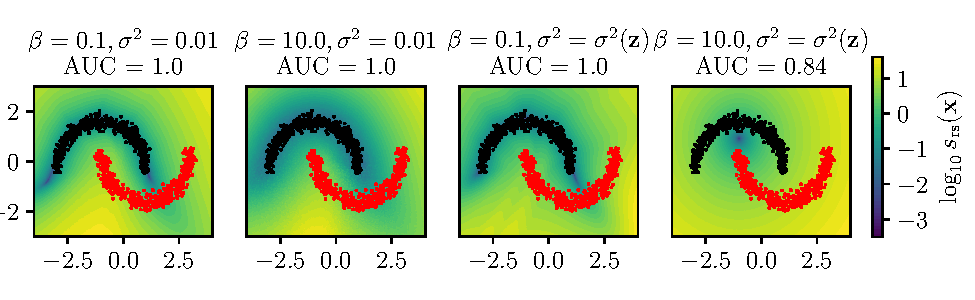
\includegraphics[scale=0.98]{data/chapter_survey/vae_examples.pdf}
\end{centering}
\caption{Anomaly detection with a VAE trained with the~\eqref{eq:betavae} objective on the \textit{two bananas} dataset with varying value of $\beta$ and different way of treating the decoder variance $\sigma^2$, where it is either considered fixed, or it is subject to optimization and funcionally dependent on the latent encoding $\vc{z}$. The contours of the anomaly score~\eqref{eq:score_sample} are shown.}
\label{fig:vae_examples}
\end{figure}

The use of the score~\eqref{eq:score_sample} is demonstrated in Fig.~\ref{fig:vae_examples}. In the plot, the difference between fixed and estimated decoder variance are explored again, similarly to Fig.~\ref{fig:betavae}. It is again shown that over-parametrizing the model might lead to undesired behaviour, as in the rightmost subplot, where the VAE collapsed into a single-modal Gaussian distribution.

\subsubsection{Practical examples}
The reason for using the VAE model instead of a reconstruction error of AE is the improved generalization that was described in the previous section. It is discussed in~\cite{dai2017hidden} that a VAE model is equivalent to a non--linear robust PCA model and is proficient at dismissing sparse outliers. The authors also make note of the fact that VAE is very efficient in pruning of unnecessary latent dimensions in case when the real latent structure has lower dimension than the chosen VAE latent space.

In~\cite{xu2018unsupervised} the authors present a so-called \textbf{DonutVAE} model with an enhanced loss function to detect anomalies in times series data. The architecture is similar to that of a vanilla VAE, but the training loss~\eqref{eq:vae_loss} is modified to consider the nature of the time series data. The authors then show that usage of this loss function improves overall results. This however has a caveat -- known anomalous samples must be available, otherwise the proposed loss is the same as~\eqref{eq:vae_loss}. Furthermore, the authors claim that using reconstruction probability~\eqref{eq:score_sample} can be seen as a weighted kernel density estimate. A similar problem is solved in~\cite{pereira2018unsupervised}, where a VAE model coupled with an LSTM recurrent neural network with attention mechanism is used for detecting anomalies in time series. Again, the model operates in the semisupervised setting, and it is able to capture the temporal structure in the data. 

In the self-adversarial Variational Autoencoder (adVAE)~\cite{wang2020advae}, an encoder-decoder pair is augmented with a transformer~\cite{vaswani2017attention}, whose goal is to simulate anomalies during training. A seeming flaw of the model is that it is trained only on normal data, and there is no link between the real and the simulated anomalies, although in the original paper, the authors claim its uperiority over a number of well-known competing methods. The sampled reconstruction error~\ref{eq:score_sample} is used as an anomaly score.

A variant of AAE is used in~\cite{leveau2017adversarial} where it is benchmarked on the MNIST problem. Standard normal distribution prior is compared to a Gaussian mixture model (GMM) latent prior and a special rejection component is introduced for representation of anomalies. In~\cite{chen2018unsupervised} the AAE model is compared to VAE on the task of detection of brain abnormalities in MRI images. The loss function of the autoencoding part is enhanced by a term $\gamma||\vc{z}-\vc{z}'||, \gamma > 0$, where $\vc{z}$ is a latent representation of a sample $\vc{x}$ and $\vc{z}'$ is the latent representation of the reconstructed sample $\vc{x}'$, which is supposed to improve consistency of the representation. The thesis~\cite{dimokranitou2017adversarial} also uses AAEs for detection of abnormalities in videos. The model presented in~\cite{pidhorskyi2018generative} uses an additional discriminator on top of the decoder in AAE to improve its reconstruction and generative properties. The model is then tested for anomaly detection on standard benchmark datasets.

Despite its name, GANomaly~\cite{akcay2018ganomaly, ahnDeepGenerativeModelsBased2020} is more related to adversarial autoencoders than to GANs. It consists of an encoder-decoder-encoder architecture with a discriminator, similar to an AAE. The anomaly score is the difference between latent representations of a sample after the first and second encoding. An upgrade to this model, skip-GANomaly~\cite{akcay2019skip}, uses skip connections in a U-Net type architecture. Here, the anomaly score is a combination of reconstruction error and feature-matching loss.

Another way of using generative autoencoders for anomaly detection is to combat the \textbf{curse of dimensionality} by employing their ability to produce a low--dimensional representation of high--dimensional data that preserves the important relations between individual datapoints. Then, an anomaly detection model (be it a generative or a classical one) can be trained on the data encoded in the latent space. This \textbf{two-stage} approach is especially useful when the target domain is image data and some kind of vectorization has to be used anyway. Usage of this technique will be demonstrated an experiment in the next chapter and it has been used in many publications~\cite{ergen2017unsupervised, yaoUnsupervisedAnomalyDetection2019, ruff2018deep, vskvara2020detection}. It is also used in~\cite{dai2019diagnosing}, where both stages are a VAE and the second stage has the same input and latent space dimensionality (therefore it does not compress data at all). Although this paper does not present an application in anomaly detection, it shows an improvement in learning of the latent space prior. The authors of~\cite{zong2018deep} couple an ordinary autoencoder with a Gaussian mixture model represented by a neural network. The AE reduces the problem dimension to help overcome the curse of dimensionality, while the GMM model serves as a density estimate in the latent space. Both the autoencoder and the GMM model are learnt jointly which improves the performance of the model. Secondly, the input of the GMM model is not only the latent representation, but also the reconstruction error of the sample. Although this model is not based on VAE, the proposed loss function can be viewed as being similar to the general form~\eqref{eq:general_wae_loss}, as it imposes some kind of structure on the distribution of encodings. 

In~\cite{ruff2018deep}, the model optimizes the projection of data (by virtue of NNs) to a new space, where they can be easily enclosed in a sphere of minimum radius. The approach presented in~\cite{vskvara2020detection, yaoUnsupervisedAnomalyDetection2019} explicitly splits the creation of the detector into two parts. It first trains a VAE (and its variants), and then it fixes the encoder. The anomaly score is calculated by a kNN \cite{vskvara2020detection} or by OC-SVM \cite{yaoUnsupervisedAnomalyDetection2019} detectors in the latent space, obtained by projecting the sample by the fixed encoder. The two-stage models can also be viewed as a kNN with a trained metric or OC-SVM with a trained kernel. The embedding can be optimized differently, for example, by enforcing the margin between anomaly candidates and normal data as done in the REPEN~\cite{pangLearningRepresentationsUltrahighdimensional2018} method, which uses an ensemble of 1NN detectors as the second stage.


\section{Normalizing flows} \label{sec:flow_models}
Generative models that are based on \textbf{normalizing flows} aim to model the data distribution $p(\vc{x})$ in a general and expressive manner. While GANs do not explicitly consider a model for $p(\vc{x})$ and only build a proxy (generator) that enables sampling, VAEs instead optimize a posterior $p_{\vc{\theta}}(\vc{x}|\vc{z})$ through a lower bound on the data log-likelihood. In this regard, normalizing flows are the most  exact in handling of the data distribution. This is at the cost of some requirements that need to be followed when building and training a normalizing flow model that will be described in the following text. Normalizing flows have been used to model complex probability distributions in multiple publications~\cite{dinh2014nice,rezende2015variational,kingma2016improved,jin2022pfvae}. Since the exact log-likelihood of a new sample is readily available when using a normalizing flow model, they have been applied to anomaly detection tasks in~\cite{yamaguchi2019adaflow, schmidtNormalizingFlowsNovelty2019, diasAnomalyDetectionTrajectory2020a, pevny2020sum,rudolph2022fully}.

A normalizing flow is a transformation $f_{\vc{\nu}}:\mathcal{Z} \rightarrow \mathcal{X}$ that can be used to express a data sample $\vc{x} \sim p(\vc{x})$ as
\begin{equation} \label{eq:flow1}
    \vc{x} = f_{\vc{\nu}}(\vc{z}), \vc{z} \sim p(\vc{z}),
\end{equation}
where $p(\vc{z})$ is the prior which has some desirable properties. The defining property of normalizing flow models, that differentiates them from VAEs and GANs, is that the transformation $f_{\vc{\nu}}$ must be invertible and both $f_{\vc{\nu}}$ and $f_{\vc{\nu}}^{-1}$ must be differentiable. This means that the dimension of $\vc{x}$ and $\vc{z}$ must be the same, so here we assume $\mathcal{Z} = \mathcal{X} = \mathbb{R}^d$. Therefore, from~\eqref{eq:flow1} and the formula for change of variables, we have
\begin{equation} \label{eq:flow2}
    p(\vc{x}) = p(\vc{z}) \left\vert \frac{\partial f_{\vc{\nu}}(\vc{z})}{\partial \vc{z}} \right\vert ^{-1} = p(f^{-1}_{\vc{\nu}}(\vc{x})) \left\vert \frac{\partial f^{-1}_{\vc{\nu}}(\vc{x})}{\partial \vc{x}} \right\vert 
\end{equation}
which contains the determinant of the square Jacobian matrix. In practice, the normalizing flow $f_{\vc{\nu}}$ is implemented as a neural network with weights $\vc{\nu}$. Notice that since it is fully invertible, we do not need an encoder-decoder pair like in a VAE. Again, like in the case of the vanilla VAE and GAN models, the prior might be e.g. $\mathcal{N}(0,\textbf{I})$. Thanks to~\eqref{eq:flow2}, the model can be directly optimized using the log-likelihood $- \ln p(\vc{x})$. When properly trained, it is possible to use a normalizing flow model to generate new samples using~\eqref{eq:flow1} or evaluate its density using~\eqref{eq:flow2}, which is the basis for anomaly detection.

One can see the transformation $f_{\vc{\nu}}$ as a process of reshaping the space $\mathbb{R}^d$ in order for $p(\vc{z})$ to closely fit $p(\vc{x})$. This process is commonly broken down into incremental steps described as a series of $K \in \mathbb{N}$ elementary invertible operations (flows)
\begin{equation} \label{eq:flow3}
    f_{\vc{\nu}} = f_{\vc{\nu},K} \circ f_{\vc{\nu},K-1} \circ \ldots \circ f_{\vc{\nu},1}
\end{equation}
which are composed together to form the full normalizing flow. This gives the model its name, as we can observe the "flow" of transformed variables
\begin{equation} \label{eq:flow4}
    \vc{z}_k = f_{\vc{\nu},k}(\vc{z}_{k-1}), k \in \hat{K}, \vc{z}_0 = \vc{z}, \vc{z}_K = \vc{x}.
\end{equation}
From~\eqref{eq:flow2}, we can express the normalizing flow objective as
\begin{equation}
    \mathcal{L}_{f} (\vc{x},\vc{\nu}) = - \ln p(\vc{x}) = -\ln p(\vc{z}) + \sum_{k=1}^K \ln \left\vert \frac{\partial f_{\vc{\nu},k}(\vc{z}_{k-1})}{\partial \vc{z}_{k-1}} \right\vert,
\end{equation}
where the inverse evaluation in the direction from $\vc{x}$ to $\vc{z}$ is given by $\vc{z}_{k-1} = f^{-1}_{\vc{\nu},k}(\vc{z}_{k})$. As mentioned earlier, this is used to train a normalizing flow model and is also a well-suited anomaly score.

The different flow models vary in the way the individual tranformations $f_{\vc{\nu},k}$ are constructed and trained, which is largely dependent on their application. In the \textbf{Non-linear Independent Component Estimator} (NICE)~\cite{dinh2014nice}, each individual flow is a called \textbf{aditive coupling layer}. It is an operation that splits the input $\vc{z}_{k-1}$ into two halves along its dimensions. The first half $\vc{z}_{k-1,1}$ remains unchanged and the second $\vc{z}_{k-1,2}$ undergoes a transformation using a parametrizable function $m$, which is a simple fully connected neural network with ReLU activations. Therefore
\begin{align}
    \vc{z}_{k,1} & = \vc{z}_{k-1,1} \\
    \vc{z}_{k,2} & = \vc{z}_{k-1,2} + m(\vc{z}_{k-1,1}), 
\end{align}
and the reverse operation is 
\begin{align}
    \vc{z}_{k-1,1} & = \vc{z}_{k,1} \\
    \vc{z}_{k-1,2} & = \vc{z}_{k,2} - m(\vc{z}_{k,1}), 
\end{align}
which is differentiable since $m$ is differentiable and its jacobian is easily computed. The \textbf{Real-valued Non-Volume Preserving} (RealNVP)~\cite{dinh2016density} is based on the NICE model and uses an \textbf{affine coupling layer}, where the second half of input dimesions undergo a scale-and-shift transformation
\begin{align}
    \vc{z}_{k,1} & = \vc{z}_{k-1,1} \\
    \vc{z}_{k,2} & = \vc{z}_{k-1,2} \odot \exp(s(\vc{z}_{k-1,1})) + t(\vc{z}_{k-1,1}), 
\end{align}
where $s,t:\mathbb{R}^d \rightarrow \mathbb{R}^{d/2}$ are again represented by neural networks. The reverse operation for the second input is 
\begin{align}
    \vc{z}_{k-1,2} & = (\vc{z}_{k,2}  - t(\vc{z}_{k,1})) \odot \exp(-s(\vc{z}_{k,1})).
\end{align}
The \textbf{Glow}~\cite{kingma2018glow} demonstrates applicability of normalizing flows to image data, which is otherwise a very difficult domain. The flow used in this model consists of invertible 1x1 convolutions and it is demonstrated that it is able to generate realistic images of celebrity faces. Some normalizing flow models use an autoregressive constraint~\cite{kingma2016improved} to represent the flow of information from the prior to the data distribution. The most prominent is the \textbf{Masked Autoregressive Flow} (MAF)~\cite{papamakariosMaskedAutoregressiveFlow2018}. A promising class of \textbf{Sum-product-Transform Networks} (SPTN)~\cite{pevny2020sum} combines normalizing flows with a graphical model. For a more complex overview and introduction to generative models based on normalizing flows, see~\cite{papamakariosNormalizingFlowsProbabilistic2019, kobyzevNormalizingFlowsIntroduction2020}. 

Although there are some applications of normalizing flows to anomaly detection~\cite{kirichenkoWhyNormalizingFlows2020, dias2020anomaly, rudolph2021same, gudovskiy2022cflow}, they are less popular than different autoencoding generative models. This might seem surprising, as they are at the same time praised for the theoretical exactness of the log-likelihood computation. However, it seems that maatching high-dimensional, complex distributions this way is very difficult and requires normalizing flow models with hundreds of flow levels. Thus, they are very slow to train on complex data, which is also due to the requirement $\text{dim}(\mathcal{Z}) = \text{dim}(\mathcal{X})$. The Glow model requires 200 million parameters optimized over 13,000 GPU-hours to achieve simillar performance to computationally much less expensive alternatives~\cite{kingma2018glow}. Still, normalizing flows present a very interesting branch of generative modeling.


% input the alfven part here

\section{Anomaly detection with generative models: practical example} \label{sec:alfven}
In this section, an application of generative modelling on a practical example is presented. It was previously published in~\cite{vskvara2020detection}. Some of the different generative autoencoders presented in Sec.~\ref{sec:vae_models} will be used to model data measured in a complex scientific experiment. Apart from the comparison of the previously presented anomaly scores, consider this to be a preliminary exploration of the two-stage modeling approach to anomaly detection described at the end of Sec.~\ref{sec:ad_genmodels}, where an autoencoding model is used to create a meaningful low-dimensional representation of complex data, and which is then coupled with some classical detector from Sec.~\ref{sec:taxonomy}. The same concept will also be further explored in Chapter~\ref{sec:chapter_sgvaegan}.

\begin{figure}[t]%[!htbp]
  \centering
  \includegraphics[scale=0.7]{data/chapter_alfven/overview.png}
  \caption{COMPASS shot 10870. Raw U-probe signal is in the upper plot. The corresponding spectrogram is below that. The score is the output of one of the tested models over the spectrogram at $f_0=0.9$ MHz and it is plotted third from the top. The highest peak around 1.1s corresponds to a detected chirping mode. A close-up of the spectrogram part containing the chirping mode as detected from the red part of the score plot is at the bottom. The size of the close-up is 128 $\times$ 311 pixels.}
  \label{fig:psd}
\end{figure}

\subsection{The application problem}
As already mentioned in the introductory chapter, physics has recently enjoyed an influx of very large amounts of data~\cite{bird2011computing,ball2010data} that needs to be processed and most importantly, from which new scientific discoveries may be extracted. This is also true for the field of plasma fusion, which pursues the goal of controlling a fusion reaction as a clean and almost inexhaustible source of energy. The ITER project~\cite{holtkamp2007overview}, which is going to be one of the largest and most complicated scientific experiments in history, is expected to produce up to 2 petabytes of data every day. This naturally calls for automatic processing of the data for a multitude of tasks, including anomaly detection. Currently, tokamaks are the state-of-the-art devices for experiments with controlled plasma fusion. In this section, an anomaly detection problem that appears during the operation of the COMPASS~\cite{panek2015status} tokamak will be dissected.

During the operation of COMPASS, \textbf{Alfv\'en eigenmodes}~\cite{markovic2015alfven, melnikov2015quasicoherent, markovic2017alfven} were observed. Alfv\'en eigenmodes are magnetic instabilities that degrade the performance of the tokamak and possibly endanger the plasma-facing components of the magnetic chamber~\cite{mett1992kinetic}. For this reason, their automatic detection is very important. Also, it may offer an opportunity for the study of their interactions with high-energy particles present in the plasma during an experiment. On COMPASS, chirping Alfv\'en eigenmodes are estimated to appear in about 0.1\% of all experiments. The primary means of their identification is a manual inspection of spectrograms drawn from the signal of certain magnetic probes, which is very time-consuming. See Fig.~\ref{fig:psd} for an example of the measured signal, a spectrogram that is derived from it, and a detected chirping Alfv\'en eigenmode. The spectrograms such as the one in Fig.~\ref{fig:psd} are large, so they are divided into patches of 128x128 pixels which is a feasible input size for current convolutional neural network architectures. It is also enough to capture most of a typical chirping mode as can be seen in the bottom plot in Fig.~\ref{fig:psd}. The patches that contain a chirping Alfv\'en eigenmode are considered to be anomalies. There are 370 labeled examples of patches with a chirping Alfv\'en eigenmode and a large database containing 33000 unlabeled (but considered normal) patches. This is a typical anomaly detection problem, where labeled anomalies are only used for evaluation and comparison of different models and the training dataset is considered to be anomaly-free.


\begin{figure}[ht]
\begin{center}
\begin{tikzpicture}[scale=1, transform shape]
  \vspace{-10cm}
  \node (image) at  (0,0) {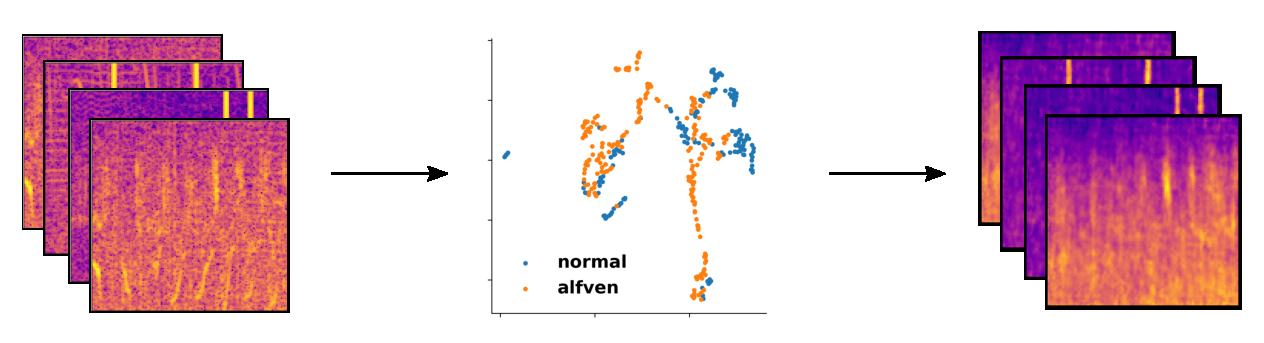
\includegraphics[width=\linewidth]{data/chapter_alfven/model_structure.pdf}};
  \node (encdim) at (-6,\capy) {$\vc{x} \in \mathbb{R}^{128\times128\times1}$};
  \node (decdim) at (6,\capy) {$\vc{x}' \in \mathbb{R}^{128\times128\times1}$};
  \node (latdim) at (0, \capy) {$\vc{z} \in \mathbb{R}^{h}$};
  \node (enc) [align=left] at (\encx, .3) {$e_{\vc{\phi}}(\vc{x})$};
  \node (dec) [align=left] at (\decx, .3) {$g_{\vc{\theta}}(\vc{z})$};
\end{tikzpicture}
\end{center}
\caption{A schematic diagram of the convolutional autoencoder used for our experiments. Spectrogram patches are encoded through several convolutional, maxpooling and dense (fully connected) layers into $h$-dimensional vectors (here $h=2$) and then decoded back with transposed convolutions and upscaling layers.}
\label{fig:alfven_ae}
\end{figure}

\subsection{The experimental setup}
Two basic experimental setups are tested in this section. Both are based on generative autoencoders from Sec.~\ref{sec:vae_models}. The basic models have similar architectures, but they differ in the probability divergences used to regularize the latent space. The KLD~\eqref{eq:vae_kld} of a VAE model is compared against the MMD~\eqref{eq:mmd}. A WAE model with a discriminator is regularized by JSD which results in the training losses~\eqref{eq:aae_loss_disc} and~\eqref{eq:aae_loss_autoencoder}. Finally, a plain AE from Sec.~\ref{sec:reconstruction_models} is included to verify that a regularized latent space is useful. The individual components of the models (encoders, decoders, discriminators) are represented by neural networks with convolutional architecture. This is the most often used architecture for image data, as several levels of convolution operations are designed to capture shift-invariant features at different scales of an image. For more technical details on the construction of the models, see~\cite{vskvara2020detection}. A schematic of a prototypical model is in Fig.~\ref{fig:alfven_ae}. The models have Gaussian encoders and decoders. The prior is either $\mathcal{N}(0,\mathbf{I})$ or Vamp, as described in Sec.~\ref{sec:wae}, and the choice is treated as a hyperparameter. Note that Vamp is only possible to use with the MMD or JSD metrics or their combination.

In the first setup, the described models are compared against each other as primary anomaly detectors in the \textbf{one class} setting. This means that they are trained on the (assumed) normal spectrogram patches and the anomaly score is the sampled reconstruction error~\eqref{eq:score_sample} in case of probabilistic autoencoders, and the reconstruction error~\eqref{eq:ae_objective} in case of the plain autoencoder model. This will test the proposed robustness of generative autoencoders.

In the second setup, the encoding capabilities of generative encoders are leveraged to create uncorrelated low-dimensional representations of spectrogram patches. This is combined with a classifier in a combined \textbf{two-stage} model. The first stage is a convolutional generative autoencoder trained with unlabeled data. Through the use of MMD or $\text{JS}_D$ measures and Vamp, a separation of the encoded data into clusters that contain similar inputs can be enforced, which makes the task of the classifier easier. The second stage is a classifier that is trained on encoded labeled data. Two different classifiers were tested. The kNN classifier, which is similar to the kNN anomaly detector described in Sec.~\ref{sec:distance_methods}, and where the score of a sample is the average label of its $k$-nearest neighbors, assuming that the label $y \in \lbrace 0,1 \rbrace$ is zero for normal samples. The GMM classifier with $M$ components was fitted on the latent representations of both labeled and unlabeled training data. Afterward, we determine one or more components of the mixture into which the positively labeled training samples are most likely to be projected via the encoder. Then, for a new sample, the score is the (average) log-likelihood of the sample in the anomalous components. 

For more details on model architecture and hyperparameters used in the experiments, see~\cite{vskvara2020detection}. For both experimental setups, 10-fold cross-validation over different splits of training and testing data was done. In the experimental results below, the models are selected using average performance on the test set. This is not ideal, as will be shown in Chapter~\ref{sec:chapter_comparison}, but here the very low number of labeled anomalies would lead to nonrobust results if the proper train/validation/test split was done, which is even more pronounced by the splitting procedure described in Sec.~\ref{sec:alfven_splits}.

\subsection{Results}
\begin{figure}
\begin{centering}
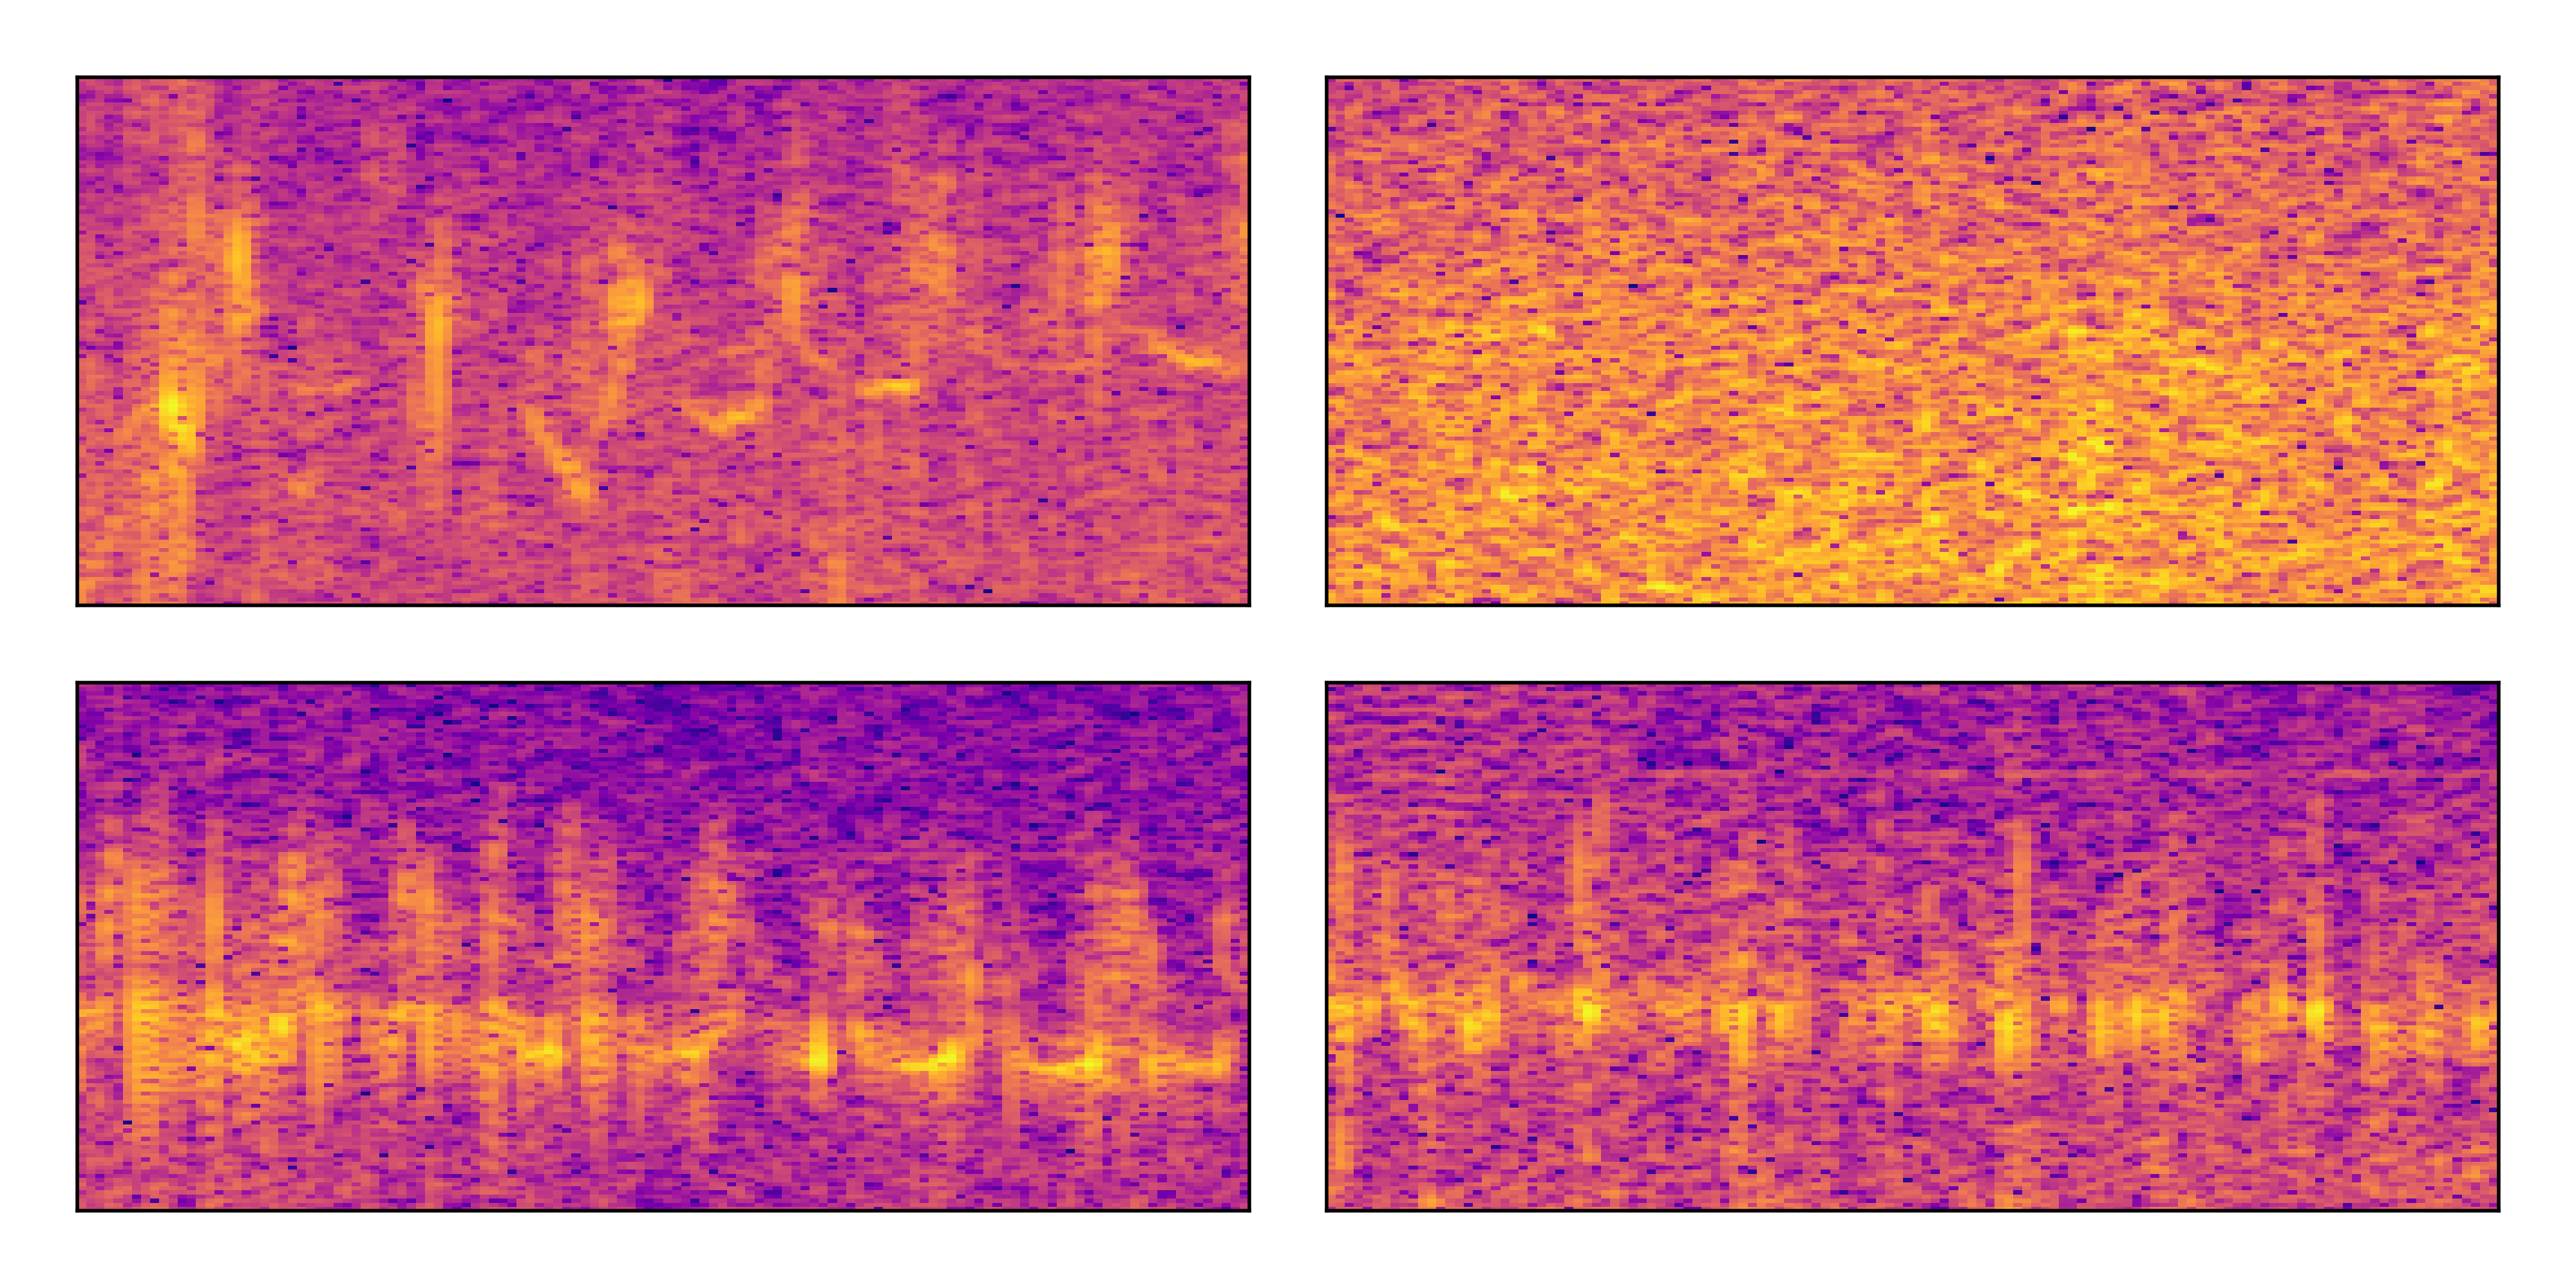
\includegraphics[scale=0.5]{data/chapter_alfven/anomalies.png}
\par
\end{centering}
\caption{Examples of spectrogram patches identified as containing a chirping
mode.}
\label{fig:alfven_patches}
\end{figure}

During the use of one of the proposed models in the production environment of the tokamak, the following workflow would be observed. A set of experiments to be analyzed would be selected. Then, the needed signals would be extracted, spectrograms computed, and divided into patches of appropriate size. These would be fed to a trained model that would produce scores to enable a ranking of the patches. Since this would produce thousands of patches and scores for each tokamak experiment, the operator would ideally only want examine a few with the highest score. The problem is illustrated in Fig.~\ref{fig:alfven_patches}, where the output of such a procedure using one of the best-performing models is shown. It contains 4 patches with the highest score, out of which 3 contain a chirping mode. It illustrates that even though the neural network encoding might be powerful, it is still basically a black box model and we need to be very careful in its evaluation. Because of this, we evaluate the model performance not only by AUC~\eqref{eq:auc}, and also by the precision@$n$ score, which is the precision at the $n$-highest scoring samples, and which is useful because it can be tuned to a certain $n$ given by the operating conditions of the tokamak. Here, we use $n=50$, which is a realistic number of samples that an operator can examine for each tokamak experiment.

\begin{table}
  \centering
  \begin{tabular}[h]{c c c c} 
\toprule
divergence & AUC & precision@50 \\ 
\midrule 
-- & 0.82 $\pm$ 0.03 & 0.86 $\pm$ 0.06 \\ 
KLD  & 0.46 $\pm$ 0.05 & 0.50 $\pm$ 0.14 \\ 
MMD  & \cellcolor{gray!45} 0.84 $\pm$ 0.03 & \cellcolor{gray!45} 0.90 $\pm$ 0.06 \\ 
JSD  & \cellcolor{gray!45} 0.84 $\pm$ 0.05 &  \cellcolor{gray!30} 0.83 $\pm$ 0.10 \\ 
MMD + JSD  & \cellcolor{gray!45} 0.84 $\pm$ 0.01 & \cellcolor{gray!15} 0.87 $\pm$ 0.01 \\ 
\bottomrule
\end{tabular}

  \caption{Results of optimization of the one class model by the divergence used in latent space regularization. The top three values are highlighted with shading. No divergence is used in a plain autoencoder with the training objective~\eqref{eq:ae_objective}.}
  \label{tab:one_class}
\end{table}

Tab.~\ref{tab:one_class} compares the performance of models in the one-class setup. The results are split by the divergence used to regularize the latent space. The difference between MMD, JSD, and their combination in terms of AUC is negligible, but MMD is slightly better than the rest in terms of precision@50. Surprisingly, vanilla VAE with KLD fails in this task altogether, which indicates that the distribution of the patches with Alfvén eigenmodes is difficult to model through a latent space with a unimodal prior.

\begin{figure}
\begin{centering}
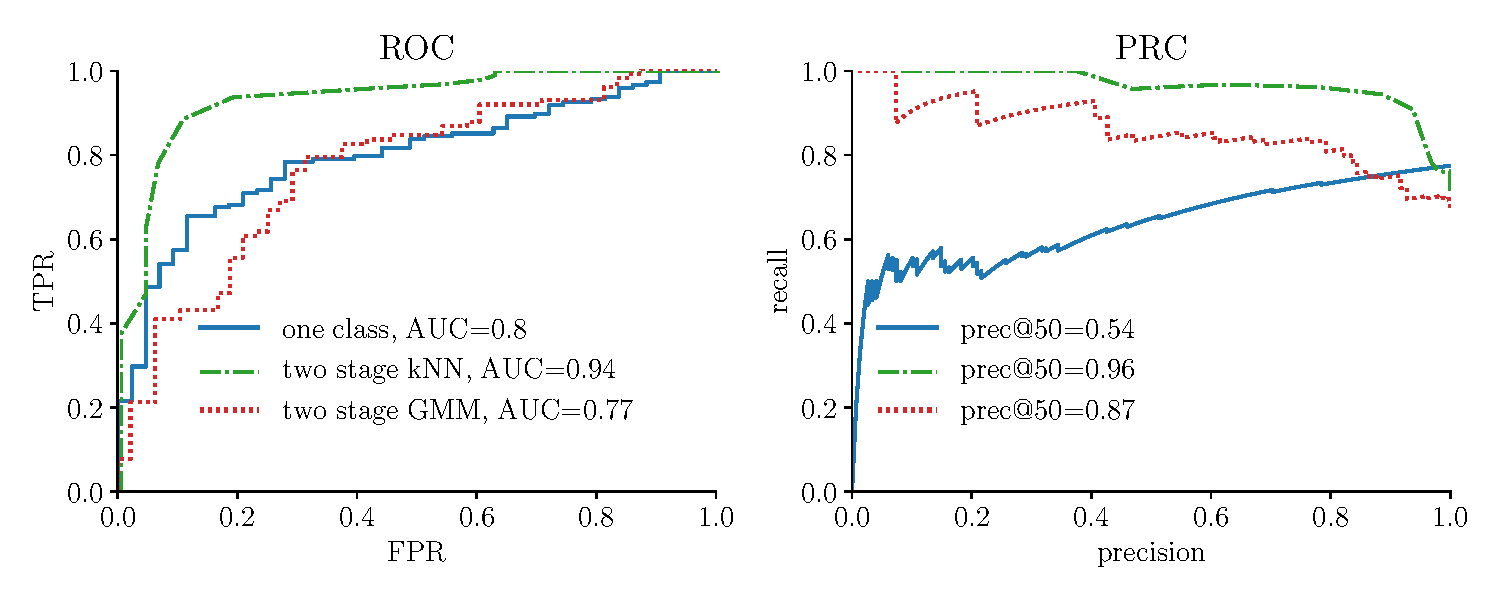
\includegraphics[scale=0.6]{data/chapter_alfven/roc_prc.pdf}
\end{centering}
\caption{ROC and PR curves of selected models. For brevity, we include the best one-class and best two-stage models in the same plot, although they are not directly comparable.}
\label{fig:roc_prc}
\end{figure}

\begin{table}
\centering
\begin{tabular}{c c c c}
	S1 divergence & S2 model & AUC & precision@50  \\
	\hline
	-- & kNN & 0.80$\pm$0.07 & 0.88$\pm$0.10 \\
	KLD & kNN & 0.80$\pm$0.08 & 0.85$\pm$0.11 \\
	MMD & kNN & \textbf{0.91$\pm$0.06} & \textbf{0.94$\pm$0.05}\\
    JSD & kNN & 0.83$\pm$0.07 & 0.87$\pm$0.10\\
    MMD + JSD & kNN & 0.86 $\pm$ 0.07 & 0.91$\pm$0.10 \\
    -- & GMM & 0.75$\pm$0.06 & 0.80$\pm$0.10\\
	KLD & GMM & 0.74$\pm$0.06 & 0.83$\pm$0.11\\
	MMD & GMM & 0.66$\pm$0.12 & 0.72$\pm$0.12\\
    JSD & GMM & 0.74$\pm$0.06 & 0.82$\pm$0.11\\
    MMD + JSD & GMM & 0.76$\pm$0.06 & 0.84$\pm$0.10
\end{tabular}
\caption{Results of hyperparameter tuning of the two-stage model across 10 cross-validation splits.}
\label{tab:alfven_results}
\end{table}

The performance of the two-stage models is summarized in Tab.~\ref{tab:alfven_results}. What is immediately obvious is that the simple kNN model is superior to the GMM approach with any encoding. Also, MMD regularization produces the best results. We might speculate that this might be due to the improved ability to produce a well-separated encoding enforced by the used prior. Fig.~\ref{fig:roc_prc} captures the ROC and PR curves for the best one-class and two-stage models.

A question one might ask is whether the use of an autoencoder is truly necessary. In the end, we are doing a projection from $d=128\times128=16384$ dimensional picture space into at most $h=64$ dimensional latent space which must naturally lead to a loss of information. As shown in Fig.~\ref{fig:patches_latent}, where $h=8$, the autoencoder is able to identify the difficult nonlinear correlations and improve the performance of a subsequent second-stage kNN model. The compression is clearly necessary for overcoming the curse of dimensionality which says that the L$_2$ distance degenerates in large dimensions. An alternative approach to overcoming the issue of large input dimension might be to train a classification convolutional neural network, which does the compression by its nature. However, such a network would be highly susceptible to overfitting since it requires a lot of labeled data that is not available.

\begin{figure}
\centering
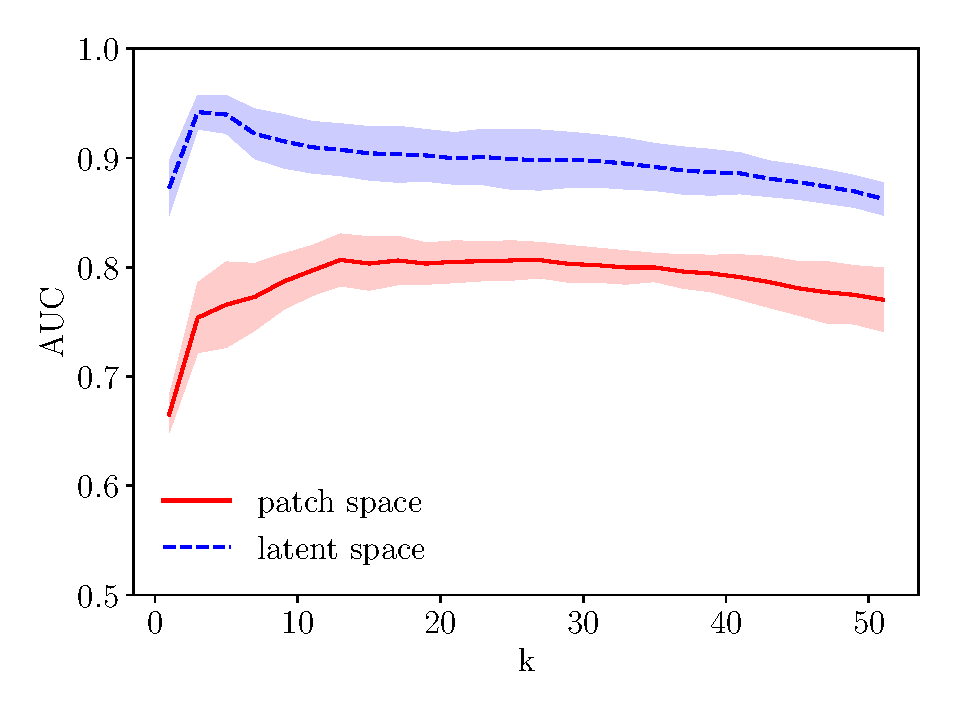
\includegraphics[scale=0.45]{data/chapter_alfven/split_patches.pdf}
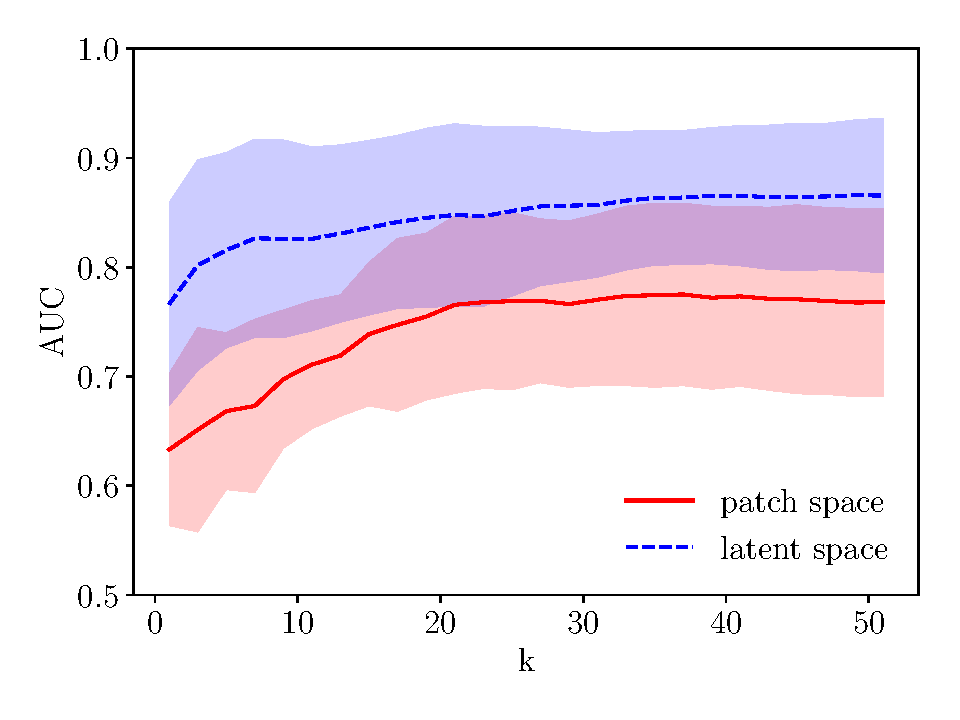
\includegraphics[scale=0.45]{data/chapter_alfven/split_spectrograms.pdf}
\caption{kNN fits for different values of $k$. The red line and band show the mean and one standard deviation bands of the resulting AUC values when kNN is fitted to the original vectorized images. The input space dimensionality is $h=16384$. The blue dashed line and band are the same quantities for a $h=8$ dimensional representation by a first-stage model. On the left, the training and testing splits were done on the level of individual patches, leading to improved performance and less variance. On the right, the split was done on the level of the original spectrograms, which is a more realistic scenario. The standard deviation and mean were computed from 10 random splits.}
\label{fig:patches_latent}
\end{figure}

\subsubsection{Influence of the train/test splitting methodology} \label{sec:alfven_splits}
At first, the splitting of testing and training labeled patches was done on the level of patches, without any regard for the spectrogram/experiment that the patch came from. It was assumed that the labeled chirping modes are homogeneous across the spectrograms. However, this turned out not to be true. Therefore, the train/test splits were done on the level of spectrograms which were then subsequently divided into patches. See Fig.~\ref{fig:patches_latent} where on the left side, the AUC curves for different values of $k$ of the kNN model are for the case when the data split was done on the level of patches. The blue line that is the result of a kNN fit peaks at $k=3$. On the other hand, there is no such peak on the right side of the figure, where splitting was done on the level of spectrograms. This indicates that the positively labeled patches in a single spectrogram are much more similar to each other than to those in different spectrograms, as only a relatively low number of neighbors is sufficient for optimal performance. Also, the variance of the right-side plots is much higher, again indicating larger differences across spectrograms. If we continued with the splitting on the level of patches, we would have a biased and too optimistic estimate of performance before using the framework in a production environment.

\subsubsection{Final remarks}
To sum up the findings from this section: generative autoencoders are a viable tool for unsupervised and semi-supervised anomaly detection. The information contained in the latent spaces is useful for anomaly detection, provided we have at least some examples of labeled anomalies. And finally, the kNN classifier proved to work very well in this simple experiment. All of these findings are going to be useful in the building of the model that is presented in Chapter~\ref{sec:chapter_sgvaegan}. 